Para la validación del prototipo se emplean los mismos bancos de prueba mencionados en la Sección (\ref{sec:PlanValidacion}), ya que no existe una diferencia sustancial que implique la necesidad de alterar dichos ensayos.

\Subsection{Validación pruebas funcionales}

Se empieza por las pruebas de \textit{T-INT-FUN-01} y \textit{T-INT-FUN-02}. Ambas pruebas se realizan a la par, no solo porque comparten el mismo banco de pruebas, sino porque se emplea el mismo sensor calibrado para la corroboración. Este sensor es capaz de medir tanto temperatura como humedad.
\begin{figure}[H]
\centering
	\begin{subfigure}{0.39\textwidth}
    	\centering
        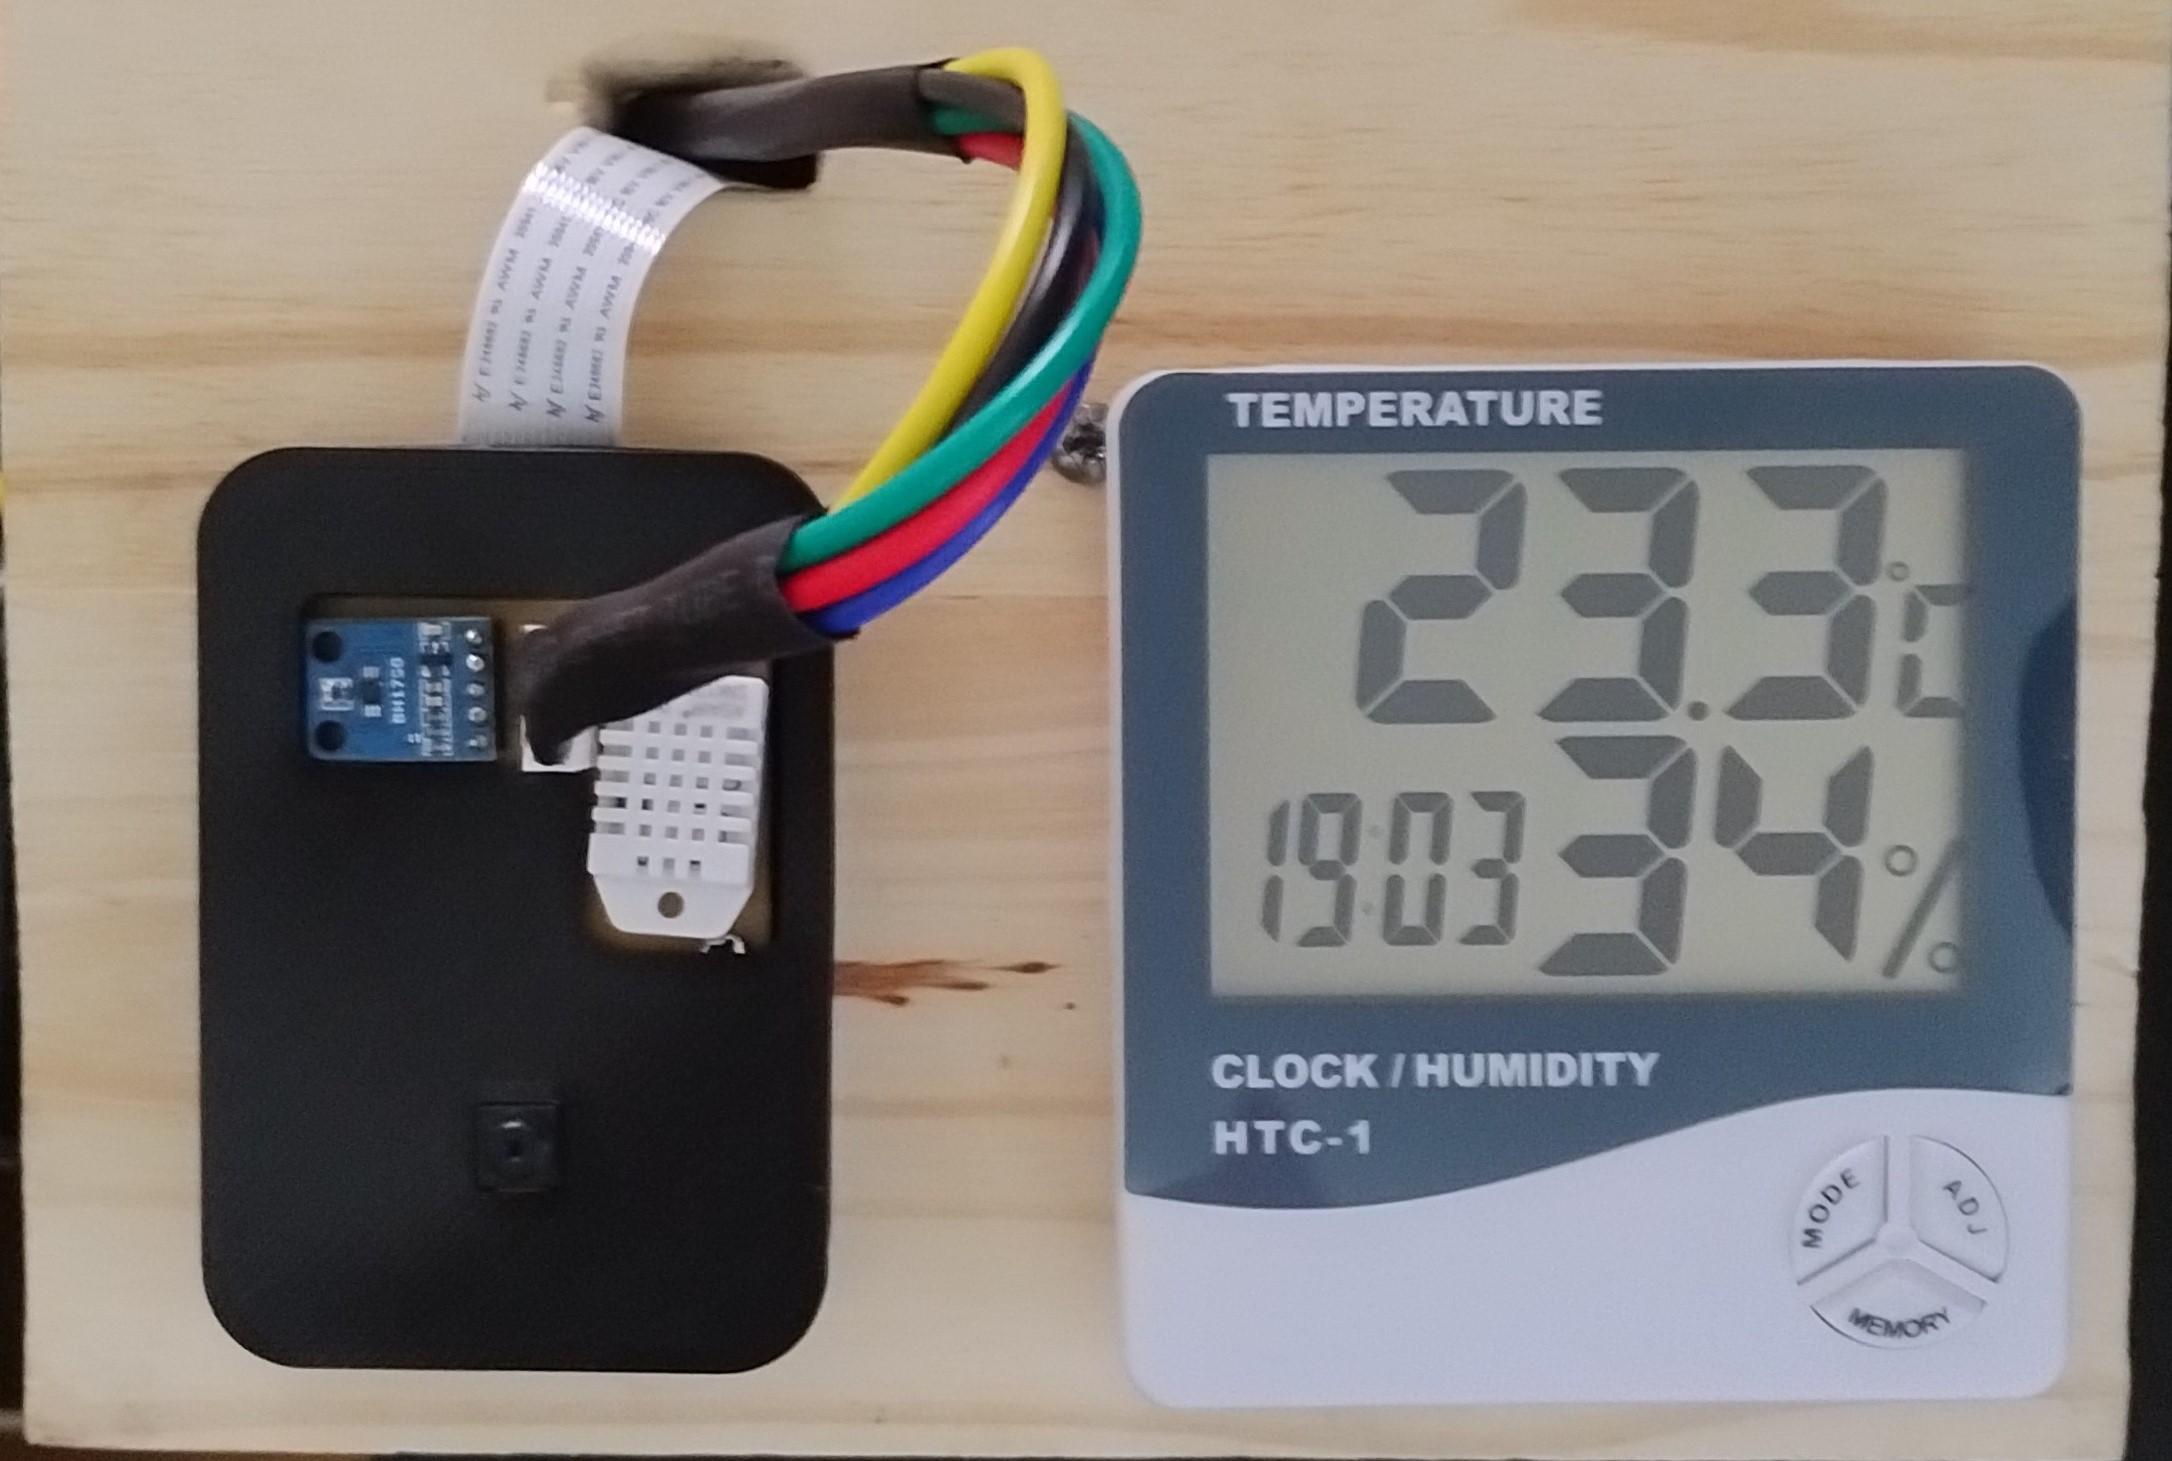
\includegraphics[width=\linewidth]{ImagenesValidacion del prototipo/T-INT-FUN-1-2-Medicion}		
		\caption{Sensores de comparación.}
	\end{subfigure}\hfill
    \begin{subfigure}{0.6\textwidth}
    	\centering
        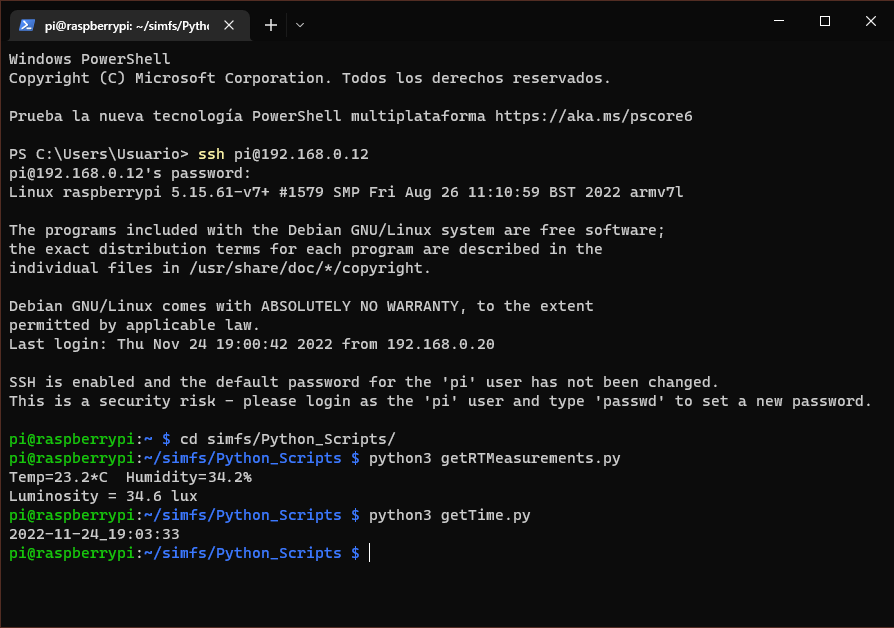
\includegraphics[width=\linewidth]{ImagenesValidacion del prototipo/T-INT-FUN-1-2}		
        \caption{Medición obtenida.}
	\end{subfigure}
	\caption{Validación de funcionalidad \textit{T-INT-FUN-01} y \textit{T-INT-FUN-02}.}
\end{figure}

De esta forma se verifica que los sensores se encuentran calibrados con un margen de error menor al máximo permitido (desviación máxima de $\pm \  0.5^o \ C$ y $\pm \ 2 \ \%$ respectivamente).

Para las validaciones del sensor de luminosidad se desarrollaron las pruebas acorde a \textit{T-INT-FUN-03}, obteniendo los resultados esperados para todos los casos, como se observa en la Figura (\ref{fig:valLum}).
\begin{figure}[H]
	\centering
    \begin{subfigure}{0.33\textwidth}
    	\centering
        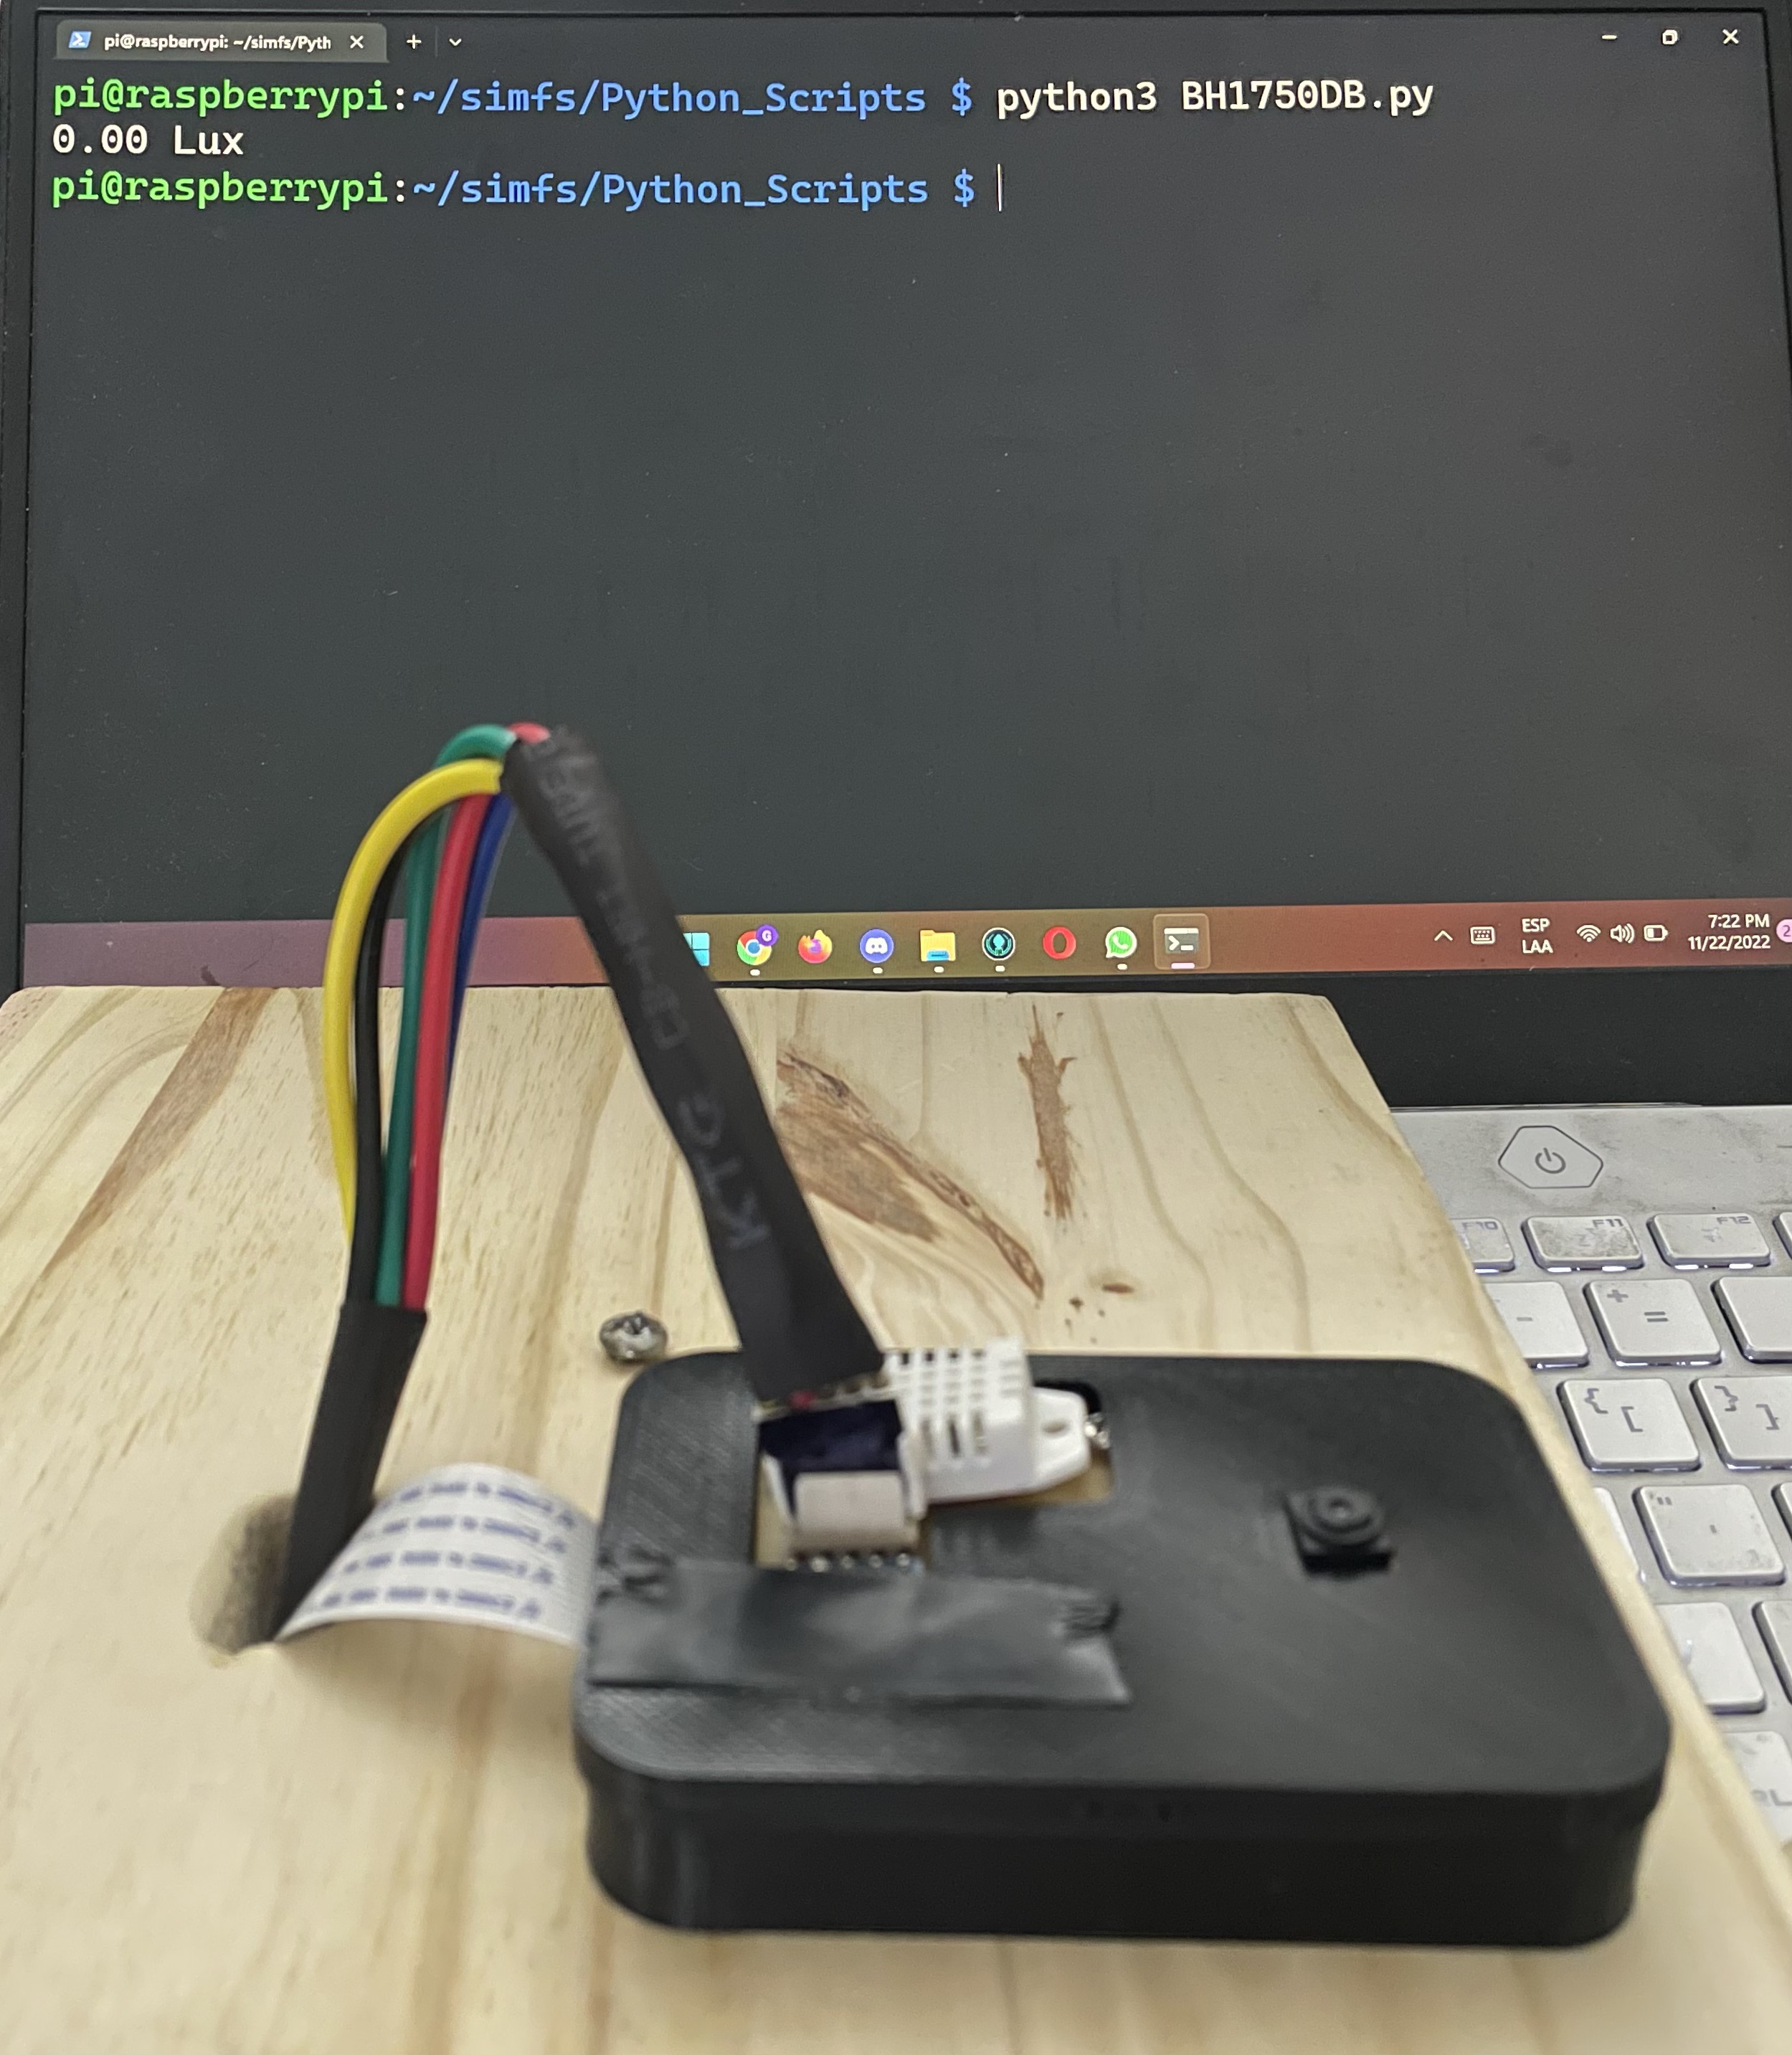
\includegraphics[width=\linewidth]{ImagenesValidacion del prototipo/TINTFUN3a}
        \caption{Sensor cubierto.}
	\end{subfigure}\hfill
    \begin{subfigure}{0.33\textwidth}
    	\centering
        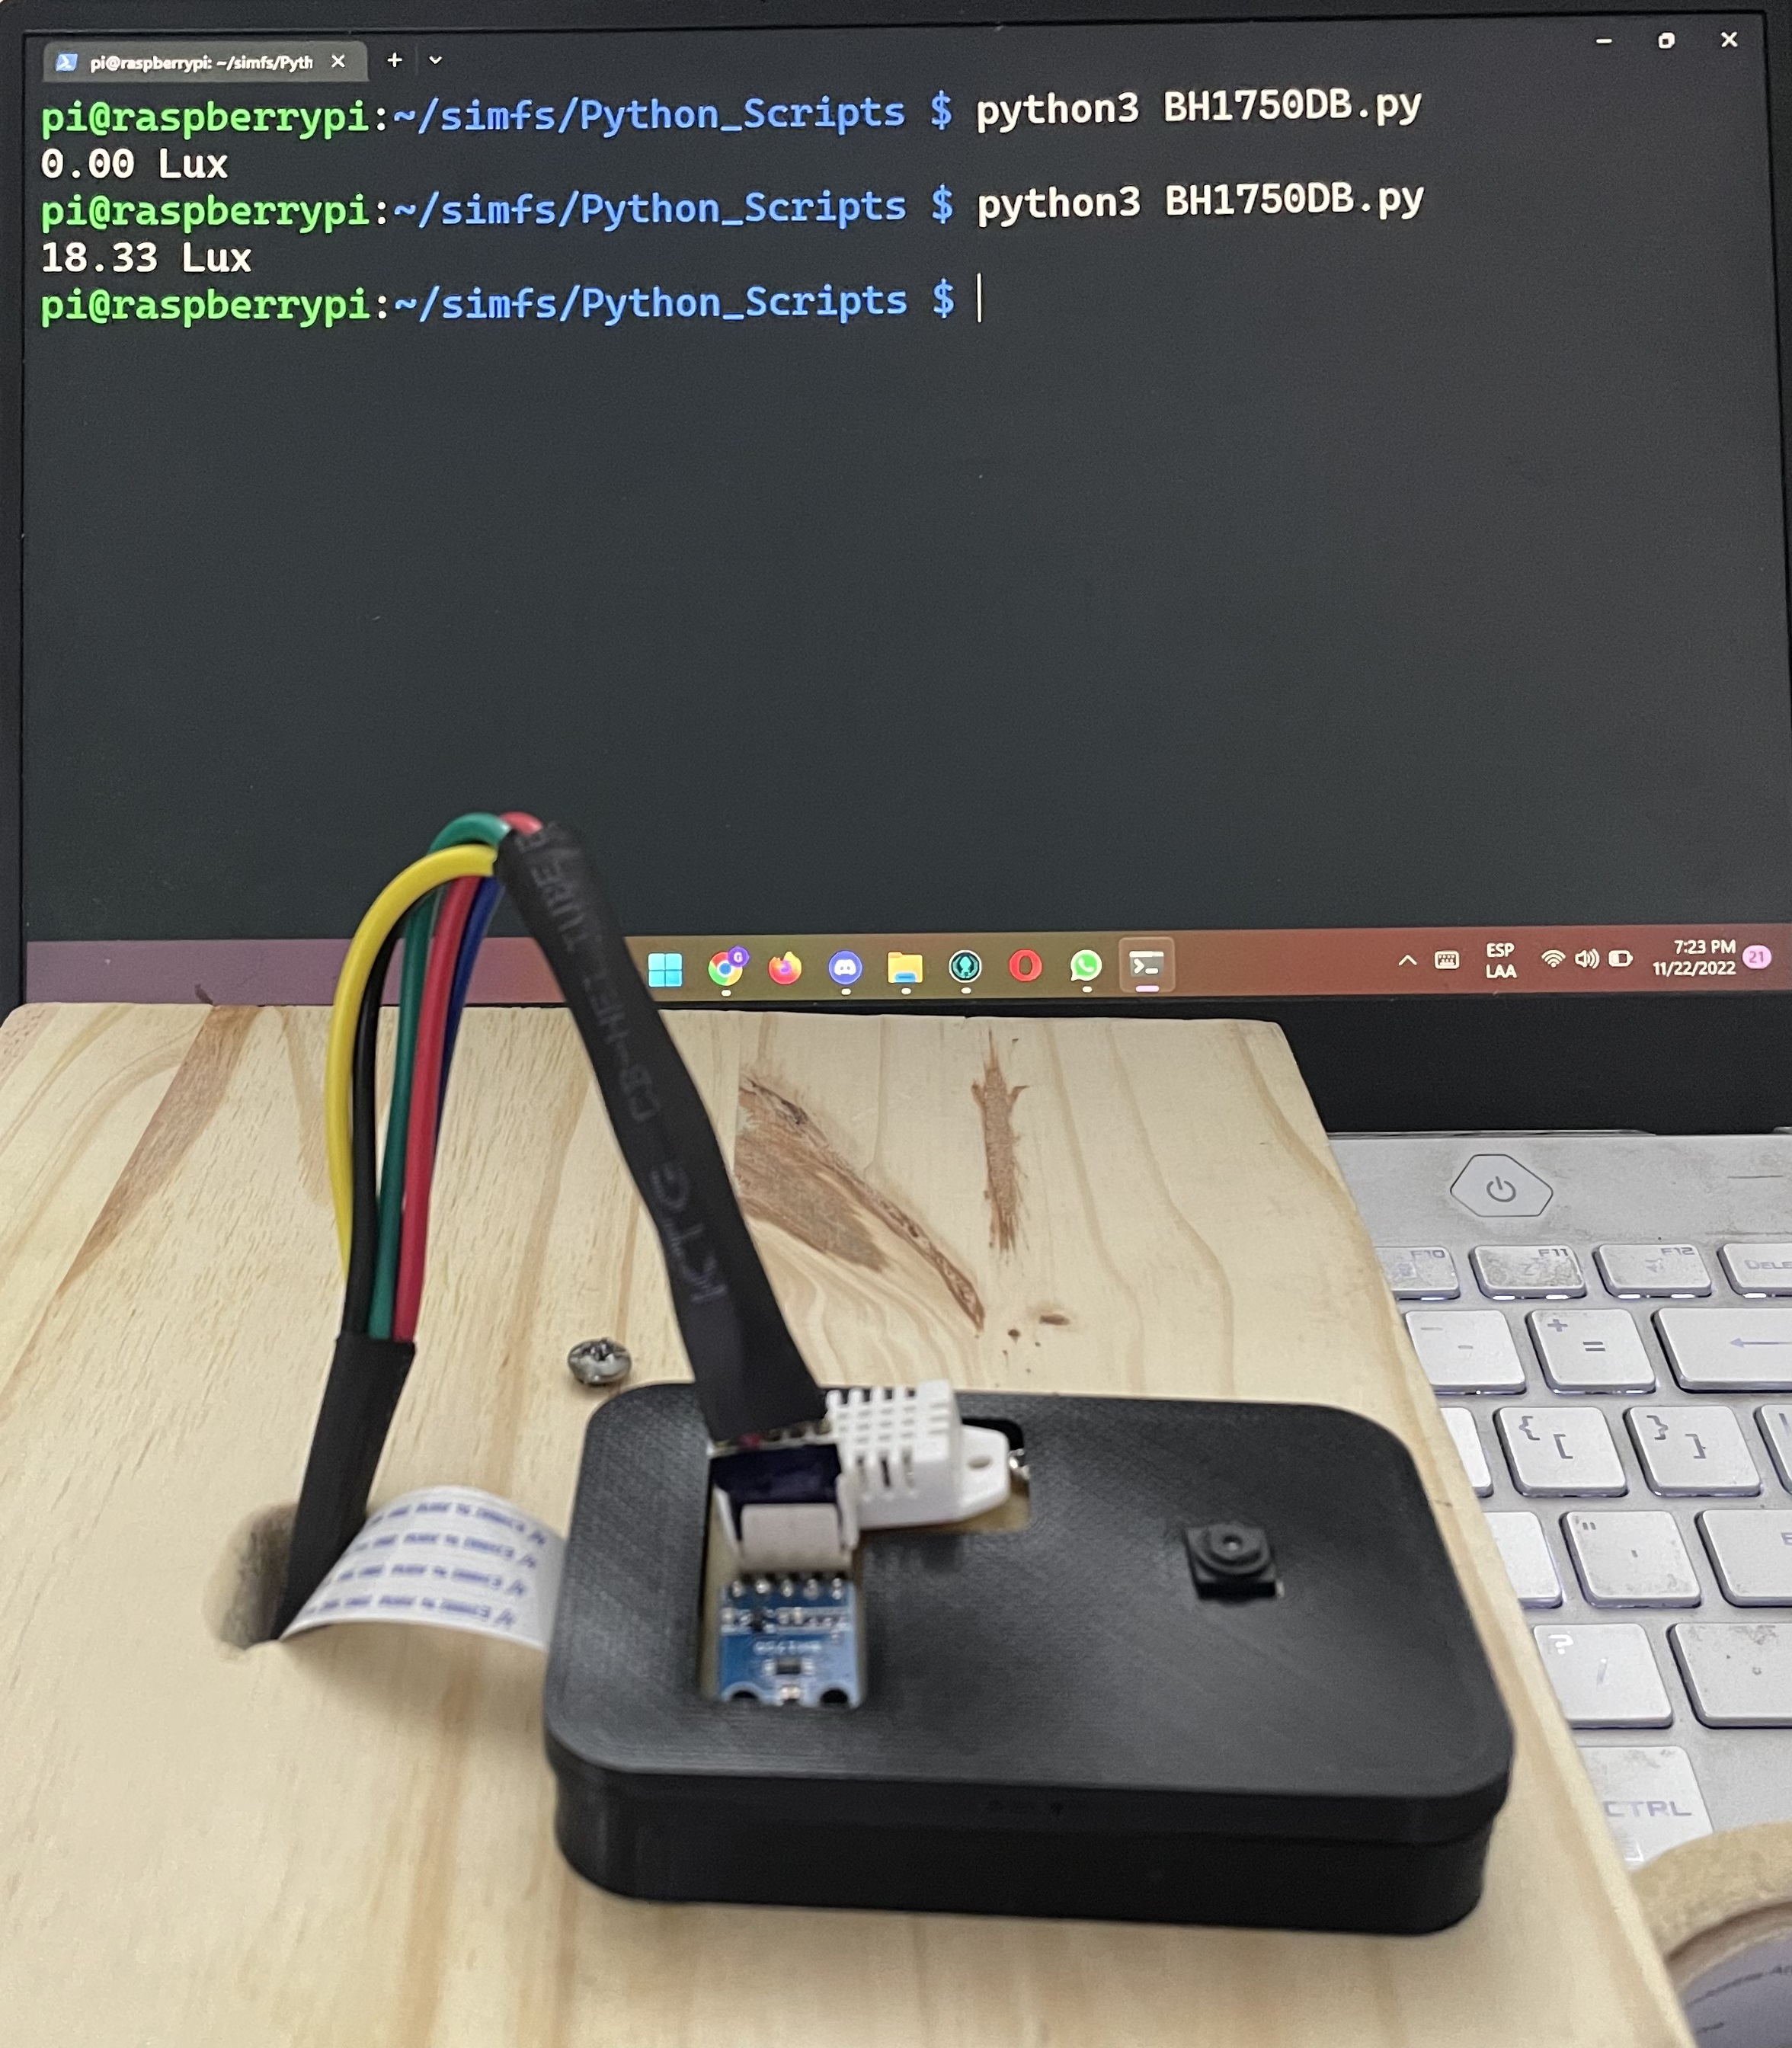
\includegraphics[width=\linewidth]{ImagenesValidacion del prototipo/TINTFUN3b}
        \caption{Sensor descubierto.}
	\end{subfigure}\hfill
    \begin{subfigure}{0.33\textwidth}
    	\centering \vspace*{3.5mm}
        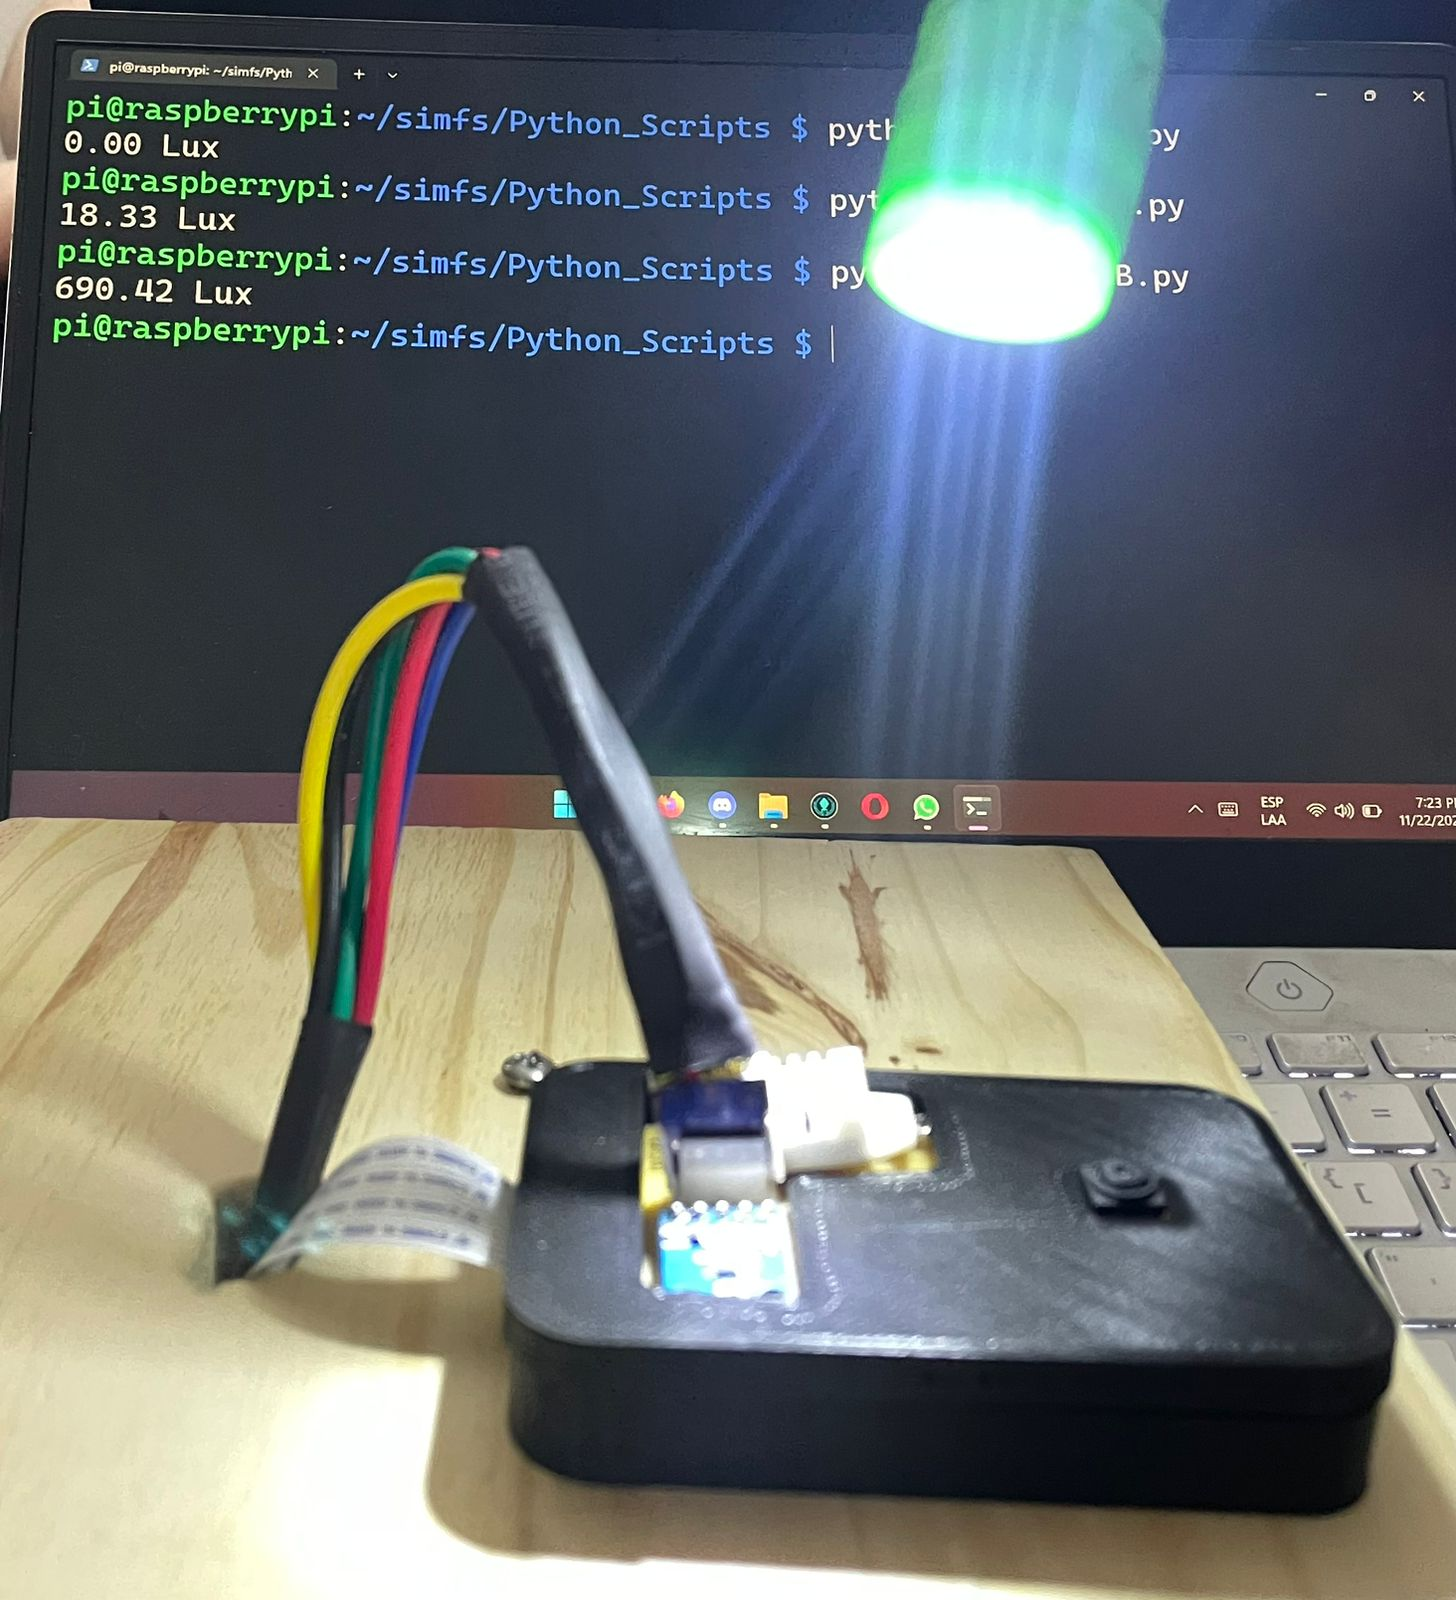
\includegraphics[width=\linewidth]{ImagenesValidacion del prototipo/TINTFUN3c}
        \caption{Sensor descubierto y apuntado con una linterna.}
	\end{subfigure}
	\caption{Validación de seguridad \textit{T-INT-FUN-03}.}
	\label{fig:valLum}
\end{figure}

Disponiendo del banco de pruebas \#3, se corroboró mediante observación los tests de funcionalidad \textit{T-INT-FUN-04} y \textit{T-INT-FUN-12}. Se garantizó que la imagen mostrada al usuario sea la adecuada y que se vea de manera fidedigna, es decir que la transmisión sea de calidad y fluida.
\begin{figure}[H]
	\centering
    	\begin{subfigure}{0.49\textwidth}
        	\centering
        	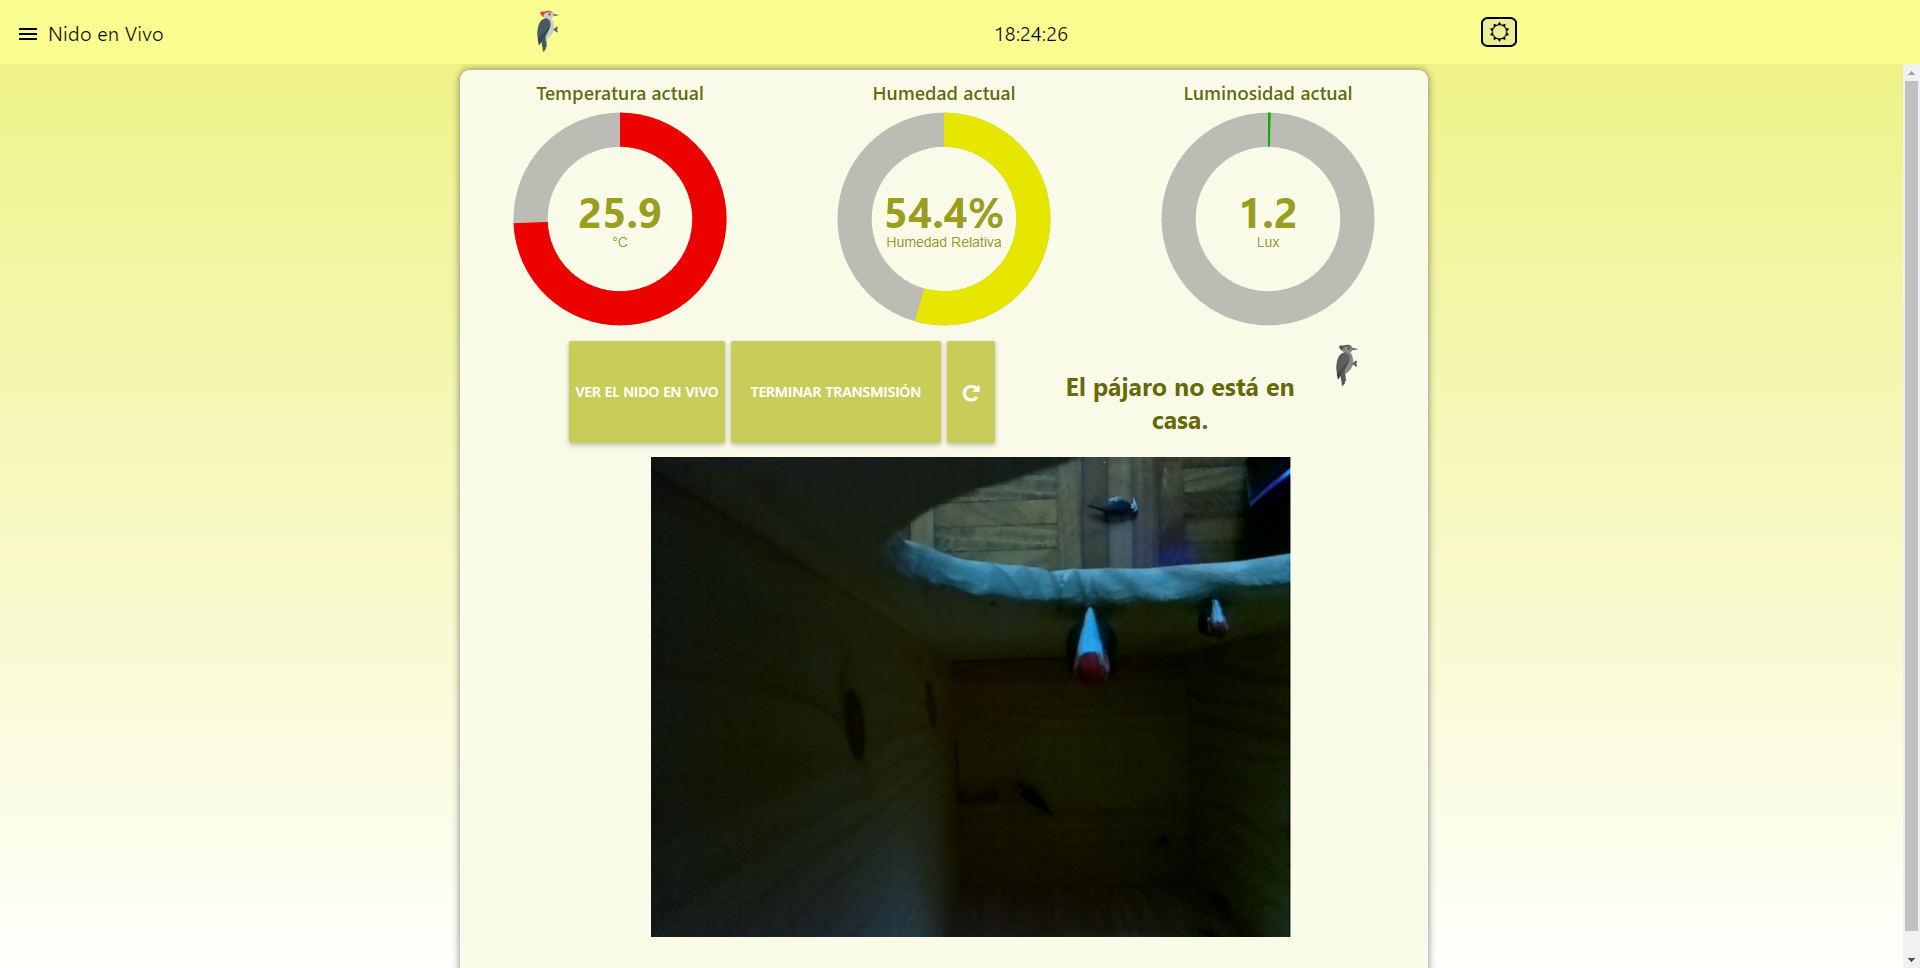
\includegraphics[width=\linewidth]{ImagenesValidacion del prototipo/t-int-fun-04-12-1}		
			\caption{Vista de la transmisión en vivo del nido.}
        \end{subfigure}\hfill
        \begin{subfigure}{0.49\textwidth}
        	\centering        	
        	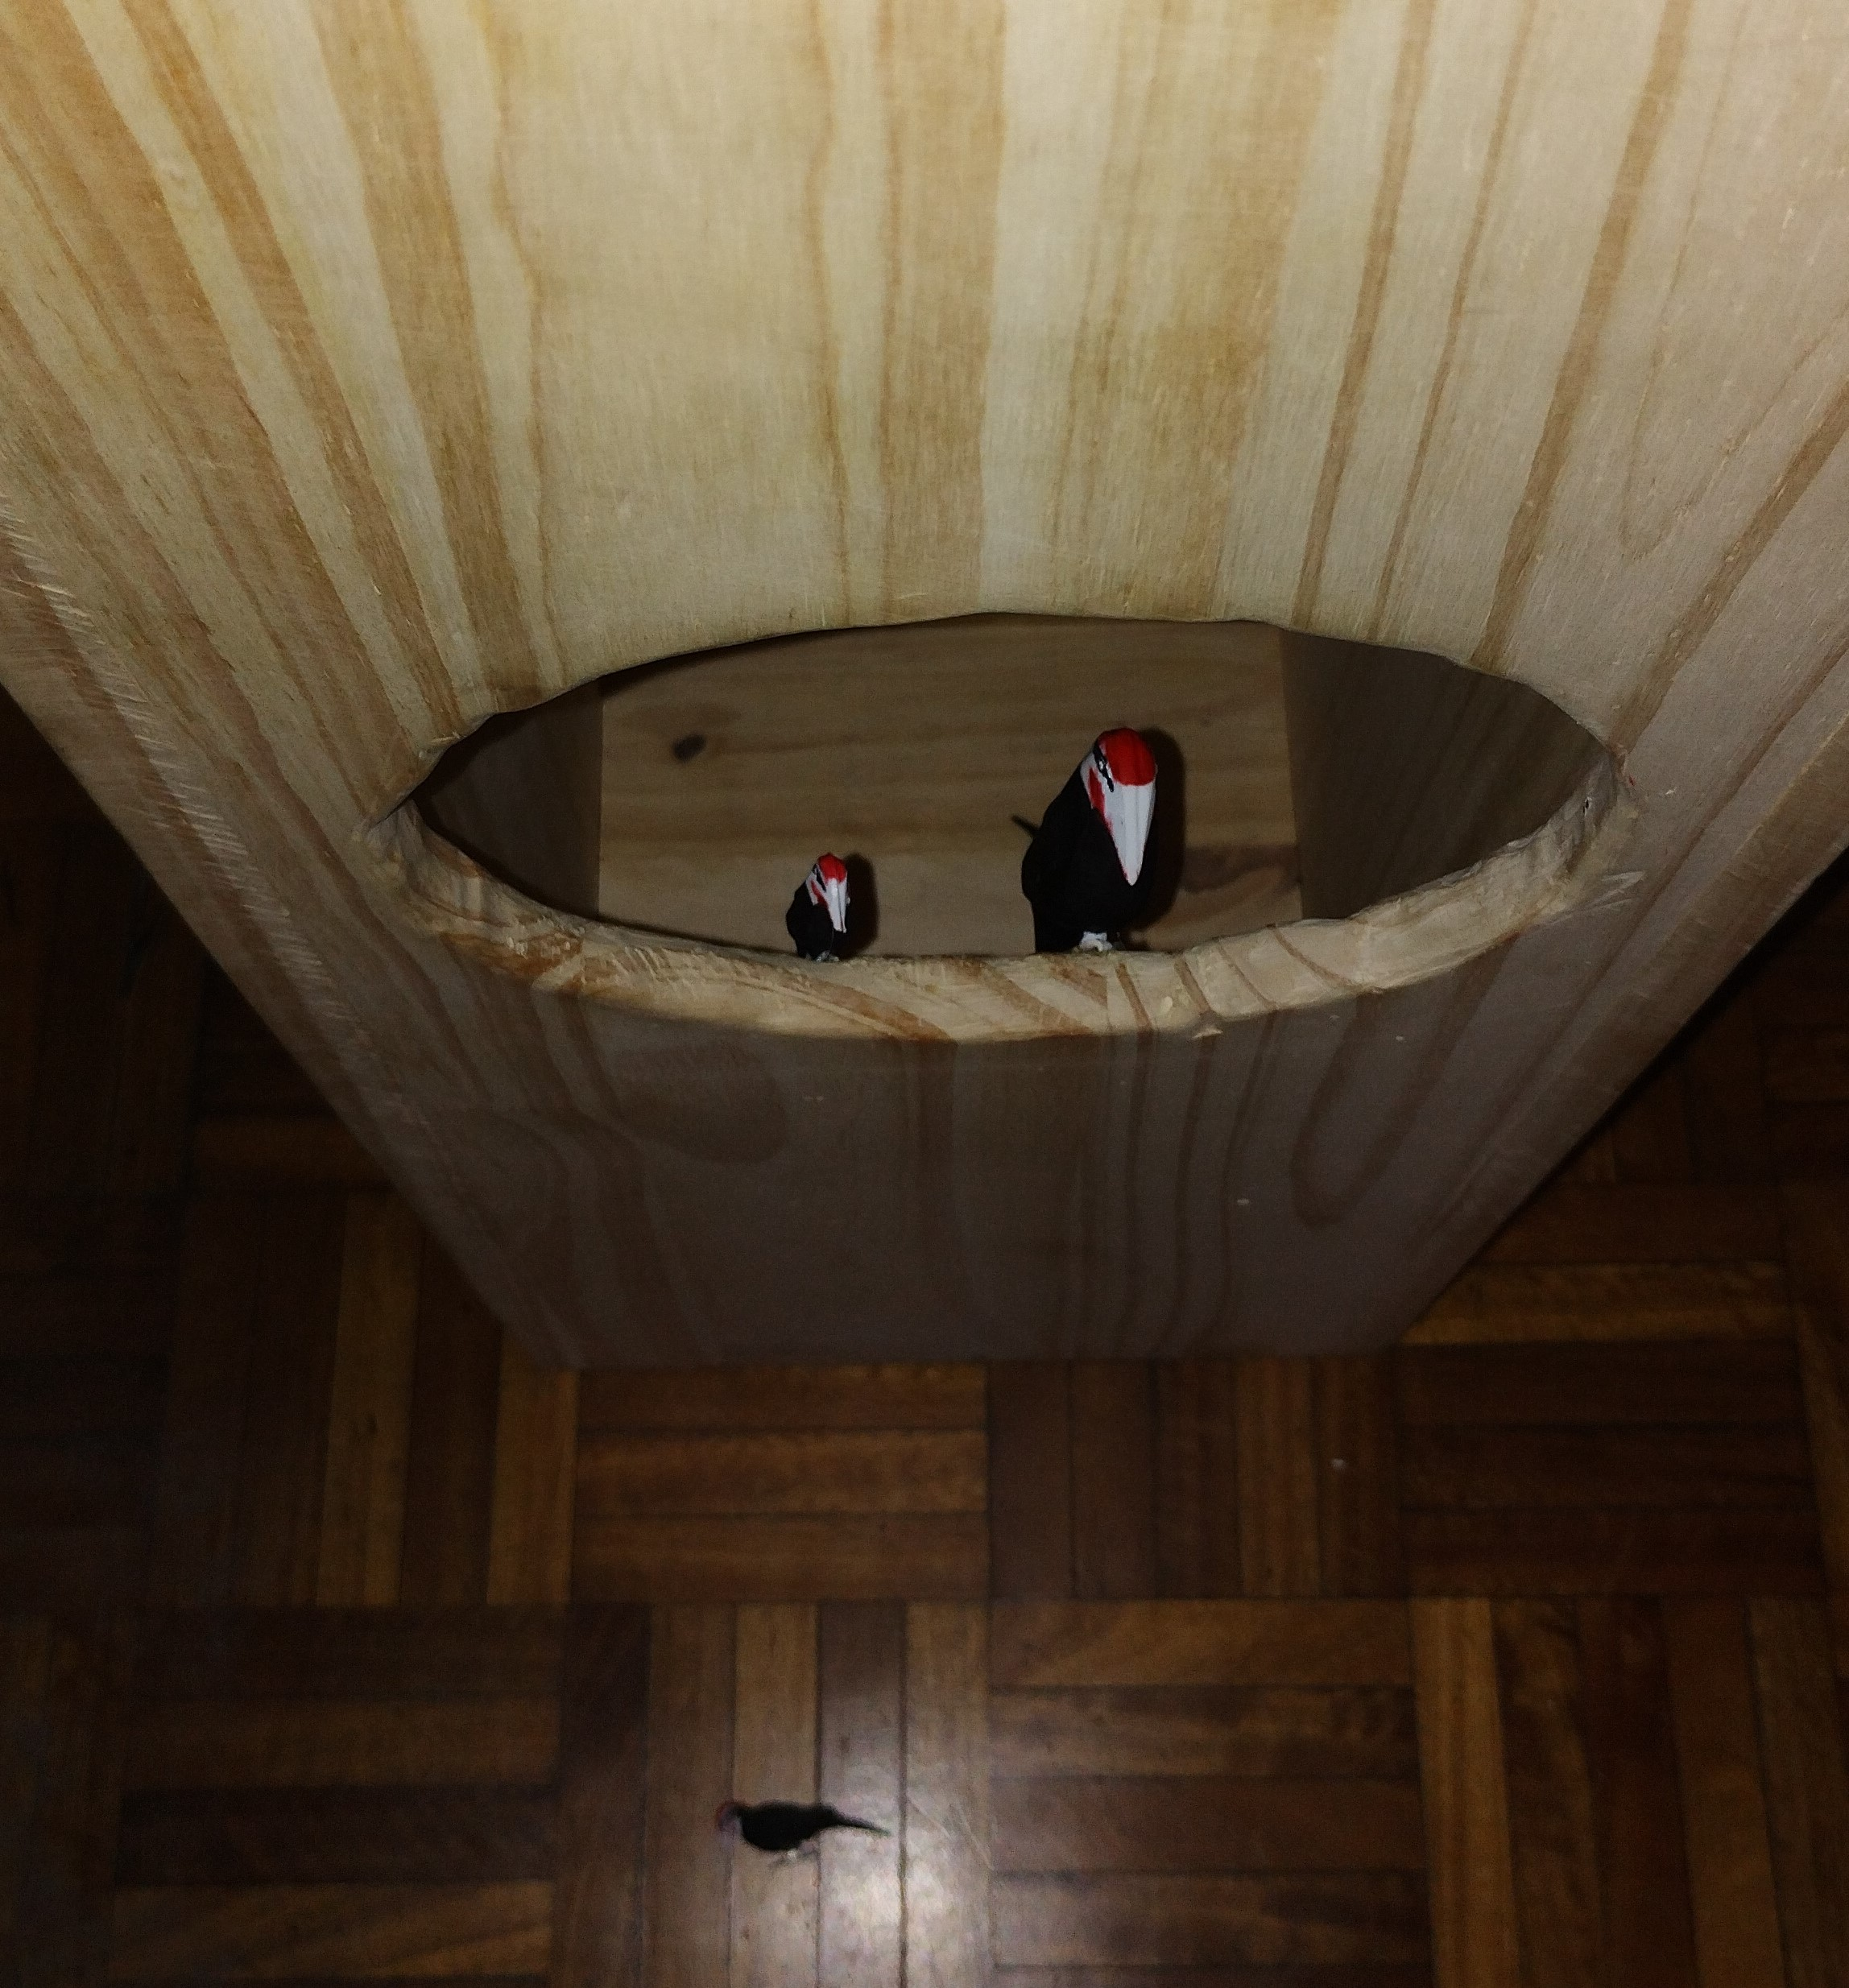
\includegraphics[width=0.5\linewidth]{ImagenesValidacion del prototipo/t-int-fun-04-12-2}
        	\caption{Imagen del exterior del nido en el momento de la trasmisión.}
        \end{subfigure}
	\caption{Validación de funcionalidad \textit{T-INT-FUN-04} y \textit{T-INT-FUN-12}.}
\end{figure}

El test de \textit{T-INT-FUN-05} se concluyó de manera satisfactoria. Resultados similares a los obtenidos se encuentran presentes en la Figura (\ref{fig:foto_camara_filtro}), donde se comparan fotos similares con y sin filtro. Por otro lado, se realiza la prueba \textit{T-INT-FUN-06}, donde se varió la posición del módulo BLE, observando los cambios de su presencia.
\begin{figure}[H]
	\centering
		\begin{subfigure}{0.49\textwidth}
			\centering
			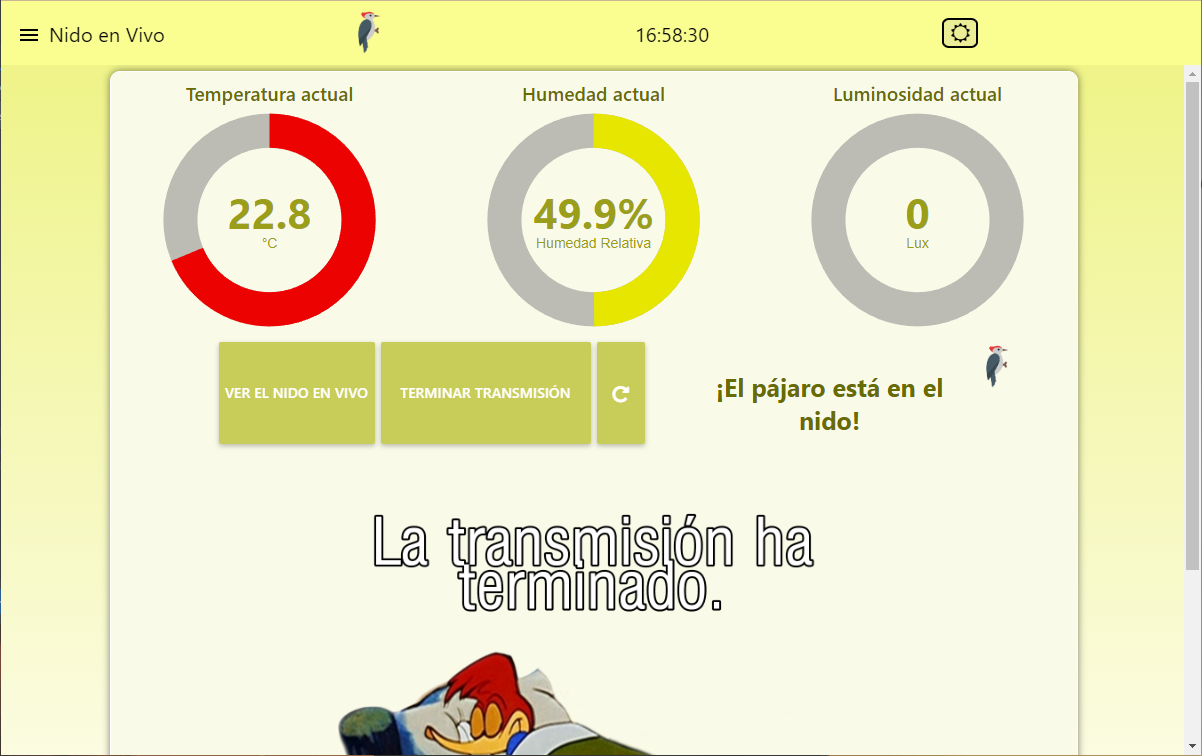
\includegraphics[width=\linewidth]{ImagenesValidacion del prototipo/T-INT-FUN-6-1}		
			\caption{\quotes{El pájaro está en el nido}.}
		\end{subfigure}\hfill
		\begin{subfigure}{0.49\textwidth}
			\centering
			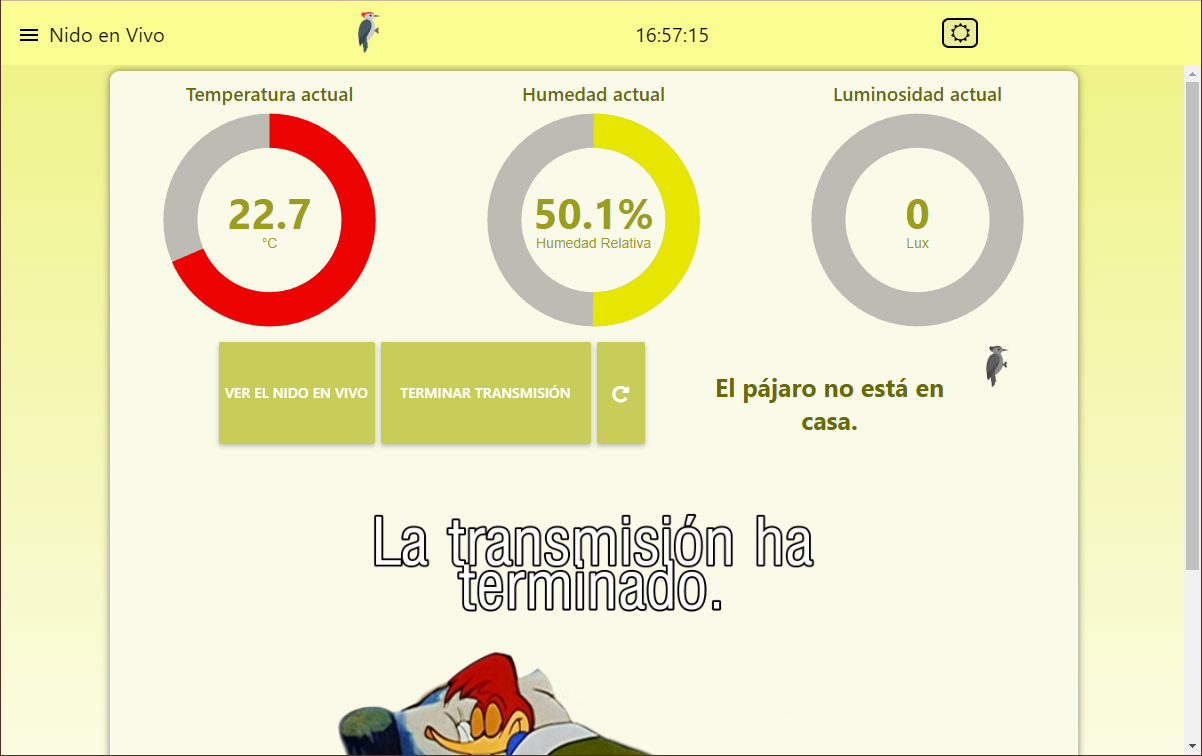
\includegraphics[width=\linewidth]{ImagenesValidacion del prototipo/T-INT-FUN-6-2}
			\caption{\quotes{El pájaro no está en casa}.}
		\end{subfigure}		
		
		\begin{subfigure}{0.49\textwidth}
			\centering
			\includegraphics[width=\linewidth]{ImagenesValidacion del prototipo/T-INT-FUN11a}	
			\caption{Beacon fuera del nido.}
		\end{subfigure}\hfill
		\begin{subfigure}{0.49\textwidth}
			\centering
			\includegraphics[width=\linewidth]{ImagenesValidacion del prototipo/T-INT-FUN11b}
		\caption{Beacon en el nido.}
		\end{subfigure}
	\caption{Variación de posición del beacon con respecto al nido.}
\end{figure}

Las validaciones a continuación están relacionadas con aspectos funcionales de los sensores. Se comienza con el periodo de muestreo de estos como indica \textit{T-INT-FUN-07}. Se puede corroborar que las mediciones son cada 5 minutos.
\begin{figure}[H]
	\centering
    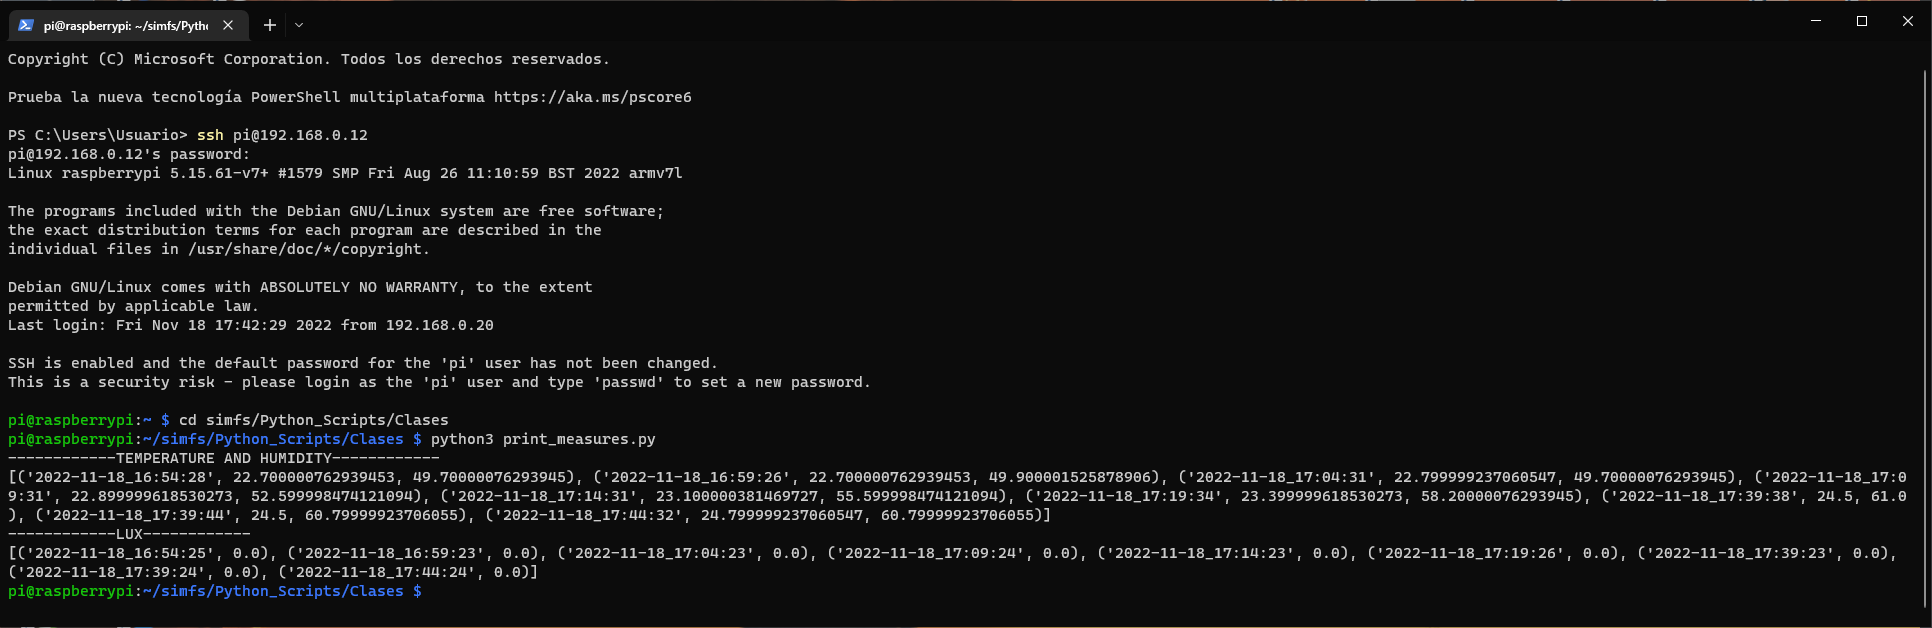
\includegraphics[width=\linewidth]{ImagenesValidacion del prototipo/T-INT-FUN-07}
	\caption{Validación de funcionalidad \textit{T-INT-FUN-07}.}
\end{figure}

Para \textit{T-INT-FUN-08} se observa que el tiempo obtenido en consola como el de la computadora, presentado en la parte inferior derecha de la imagen, coinciden. Es por esto que se considera que la prueba concluyó de manera exitosa.
\begin{figure}[H]
	\centering
    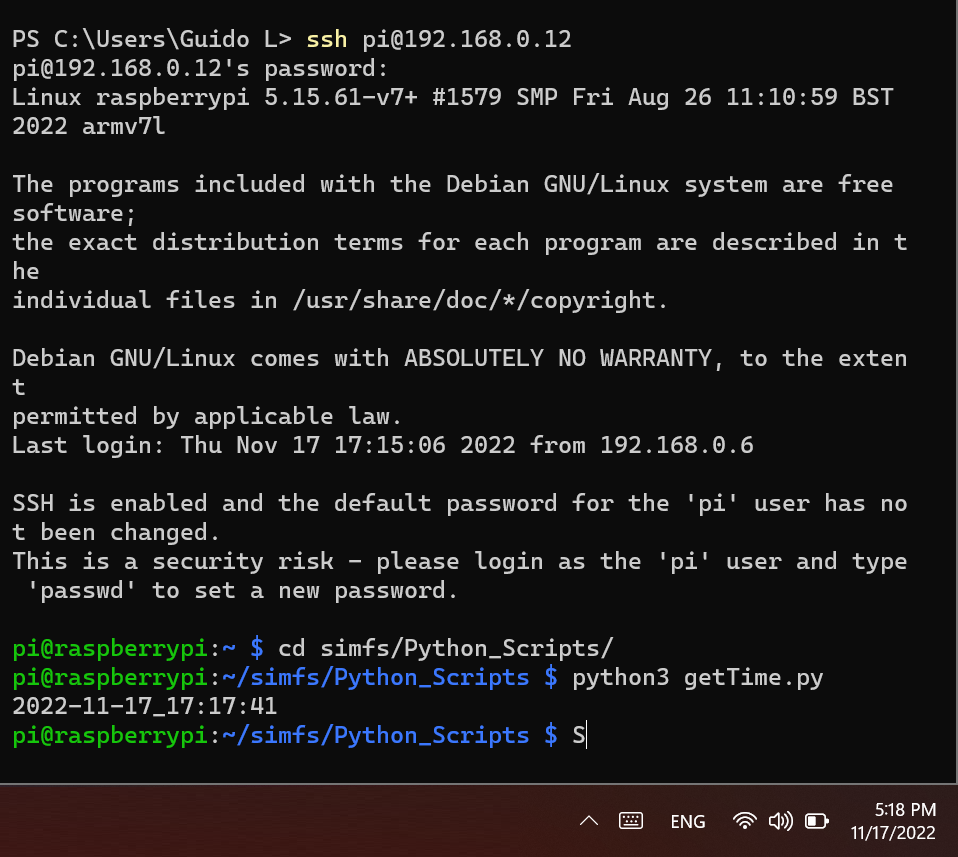
\includegraphics[width=0.8\linewidth]{ImagenesValidacion del prototipo/TINTFUN8}
	\caption{Validación de funcionalidad \textit{T-INT-FUN-08}.}
\end{figure}

La siguiente prueba corresponde a \textit{T-INT-FUN-09}. En esta se desenergiza la \rspi, y luego de esperar el tiempo apropiado, se la energiza nuevamente corroborando que la hora correspondiente al módulo RTC sea correcta.
\begin{figure}[H]
	\centering
	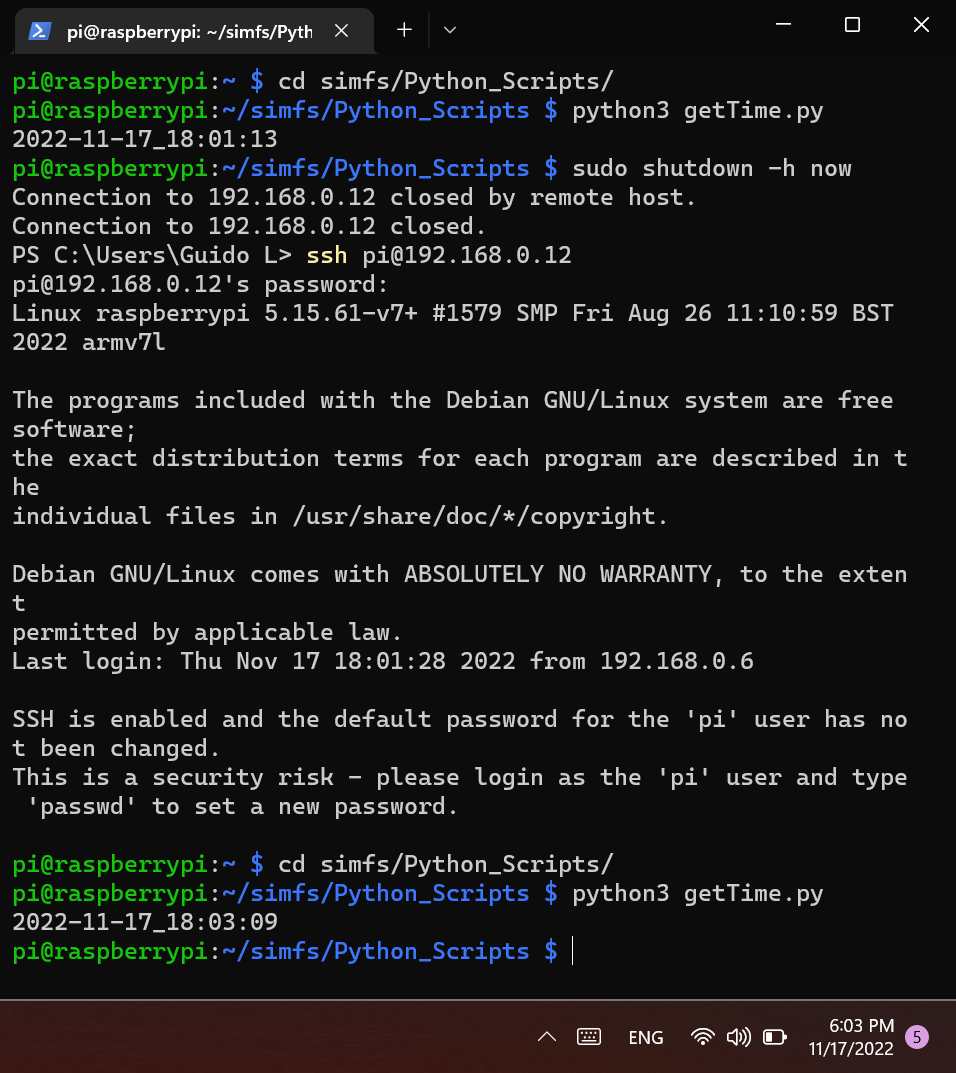
\includegraphics[width=0.8\linewidth]{ImagenesValidacion del prototipo/TINTFUN9}
	\caption{Validación de funcionalidad \textit{T-INT-FUN-09}.}
\end{figure}

\Subsection{Validación Pruebas de Comunicación 1}
\textit{T-INT-COM1-01} se efectúa disponiendo del banco de pruebas número \#3. Se emplea un dispositivo de comunicación mediante protocolo BLE. Se observa en las diversas consolas que no solo se efectúa la transmisión de datos, sino que el archivo no sufre ninguna pérdida de paquetes ya que ambos hash coinciden.
\begin{figure}[H]
	\centering
	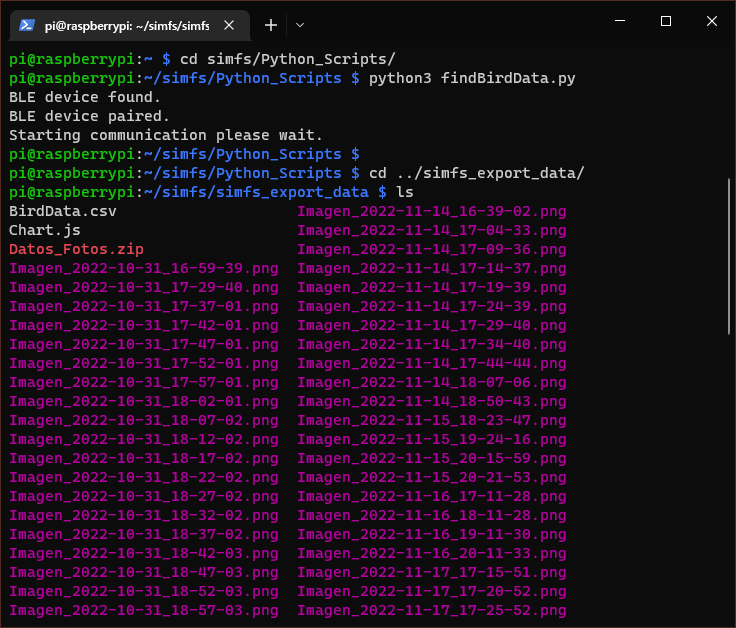
\includegraphics[width=0.8\linewidth]{ImagenesValidacion del prototipo/BirdData2}
	\caption{Consola del lado del receptor \rspi .}
\end{figure}
\begin{figure}[H]
	\centering
	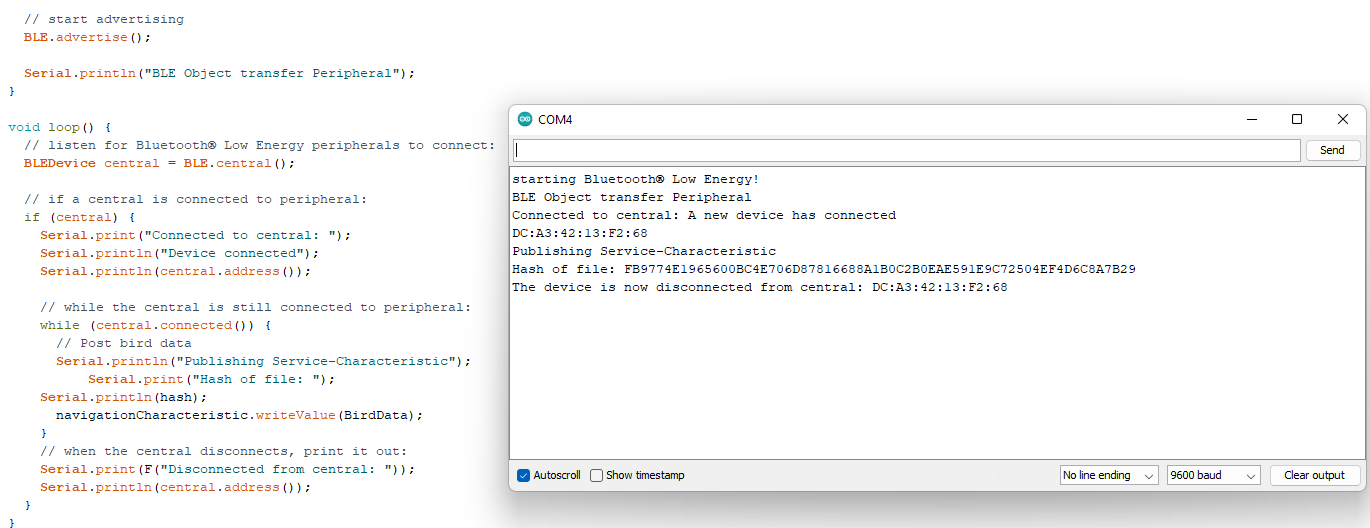
\includegraphics[width=\linewidth]{ImagenesValidacion del prototipo/T-int-com1-1-Arduino}
	\caption{Consola del lado del transmisor \textit{BPS}}
\end{figure}
Se realizó la prueba acorde a \textit{T-INT-COM1-02}, donde se obtuvieron mediciones a distintas distancias, variando entre 1 y 30 metros. Se obtuvieron resultados satisfactorios, por lo que la prueba es superada con especificaciones incluso superiores a las definidas.
\begin{figure}[H]
	\centering
	\begin{subfigure}{0.3\textwidth}
		\centering
		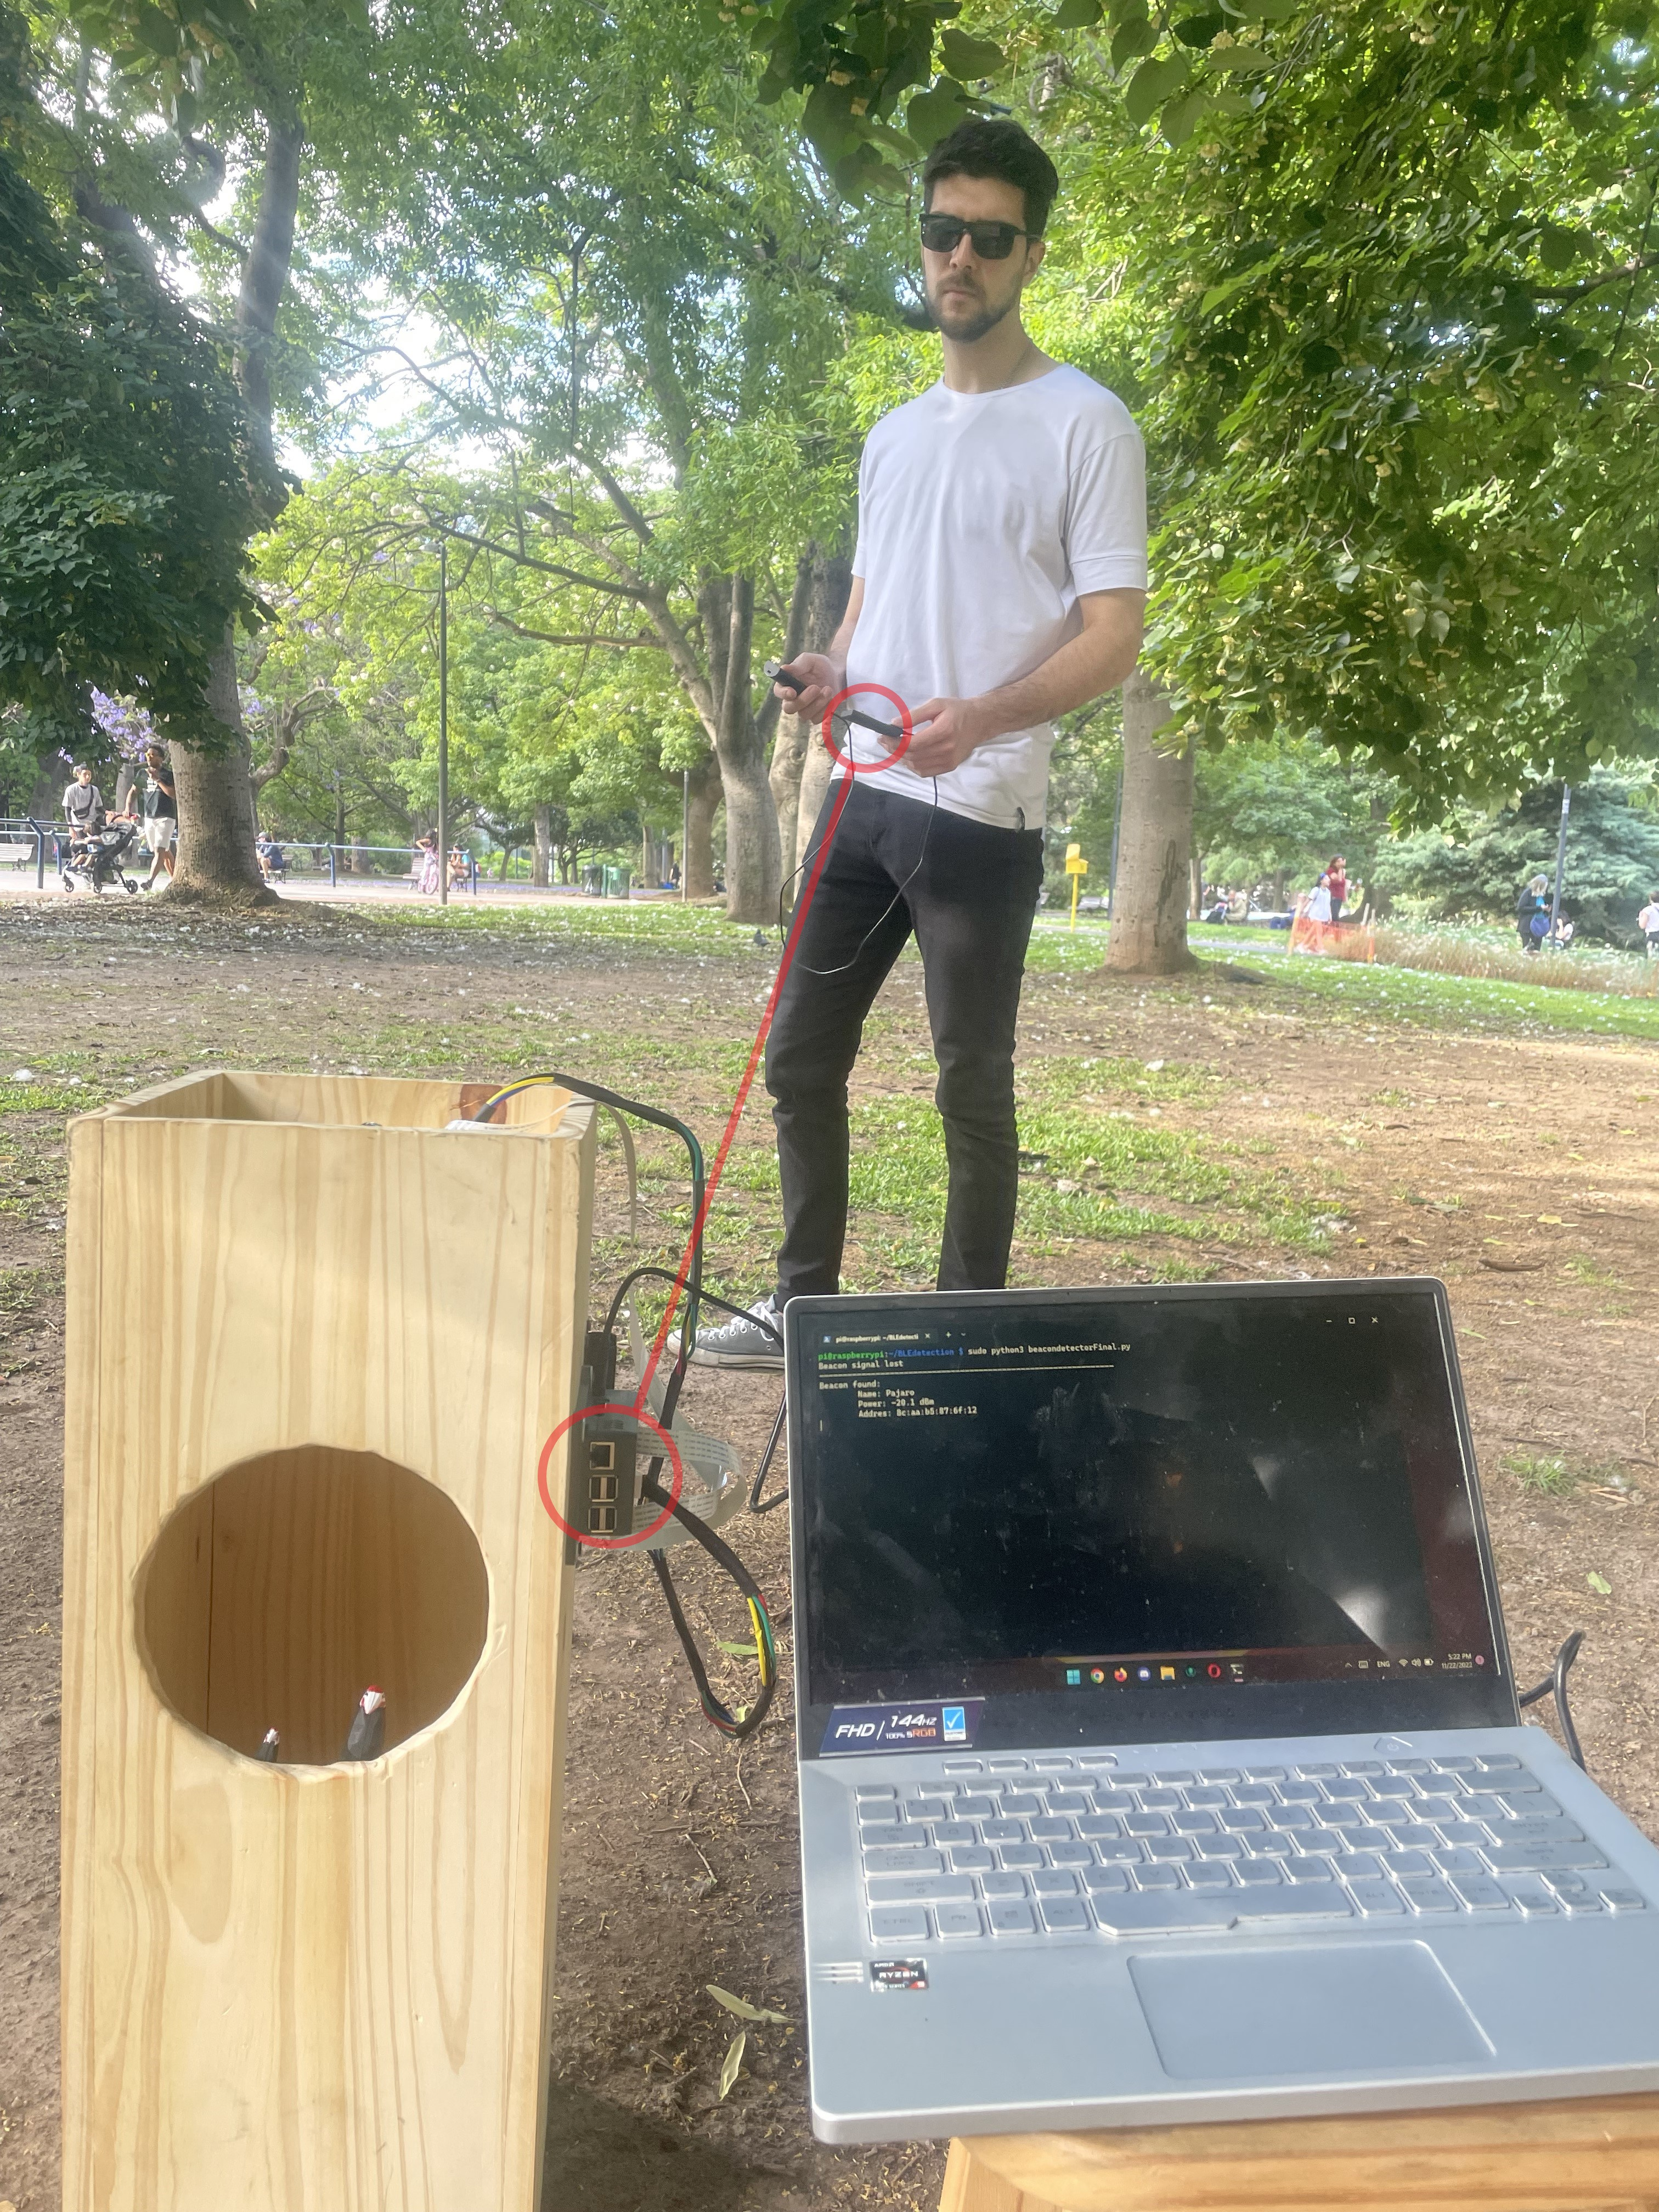
\includegraphics[width=\linewidth]{ImagenesValidacion del prototipo/TINTCOM12a}
		\caption{Distancia de 1 metro.}
	\end{subfigure}	
\end{figure}
\begin{figure}[H]
	\centering
	\ContinuedFloat
	\begin{subfigure}{0.3\textwidth}
		\centering
		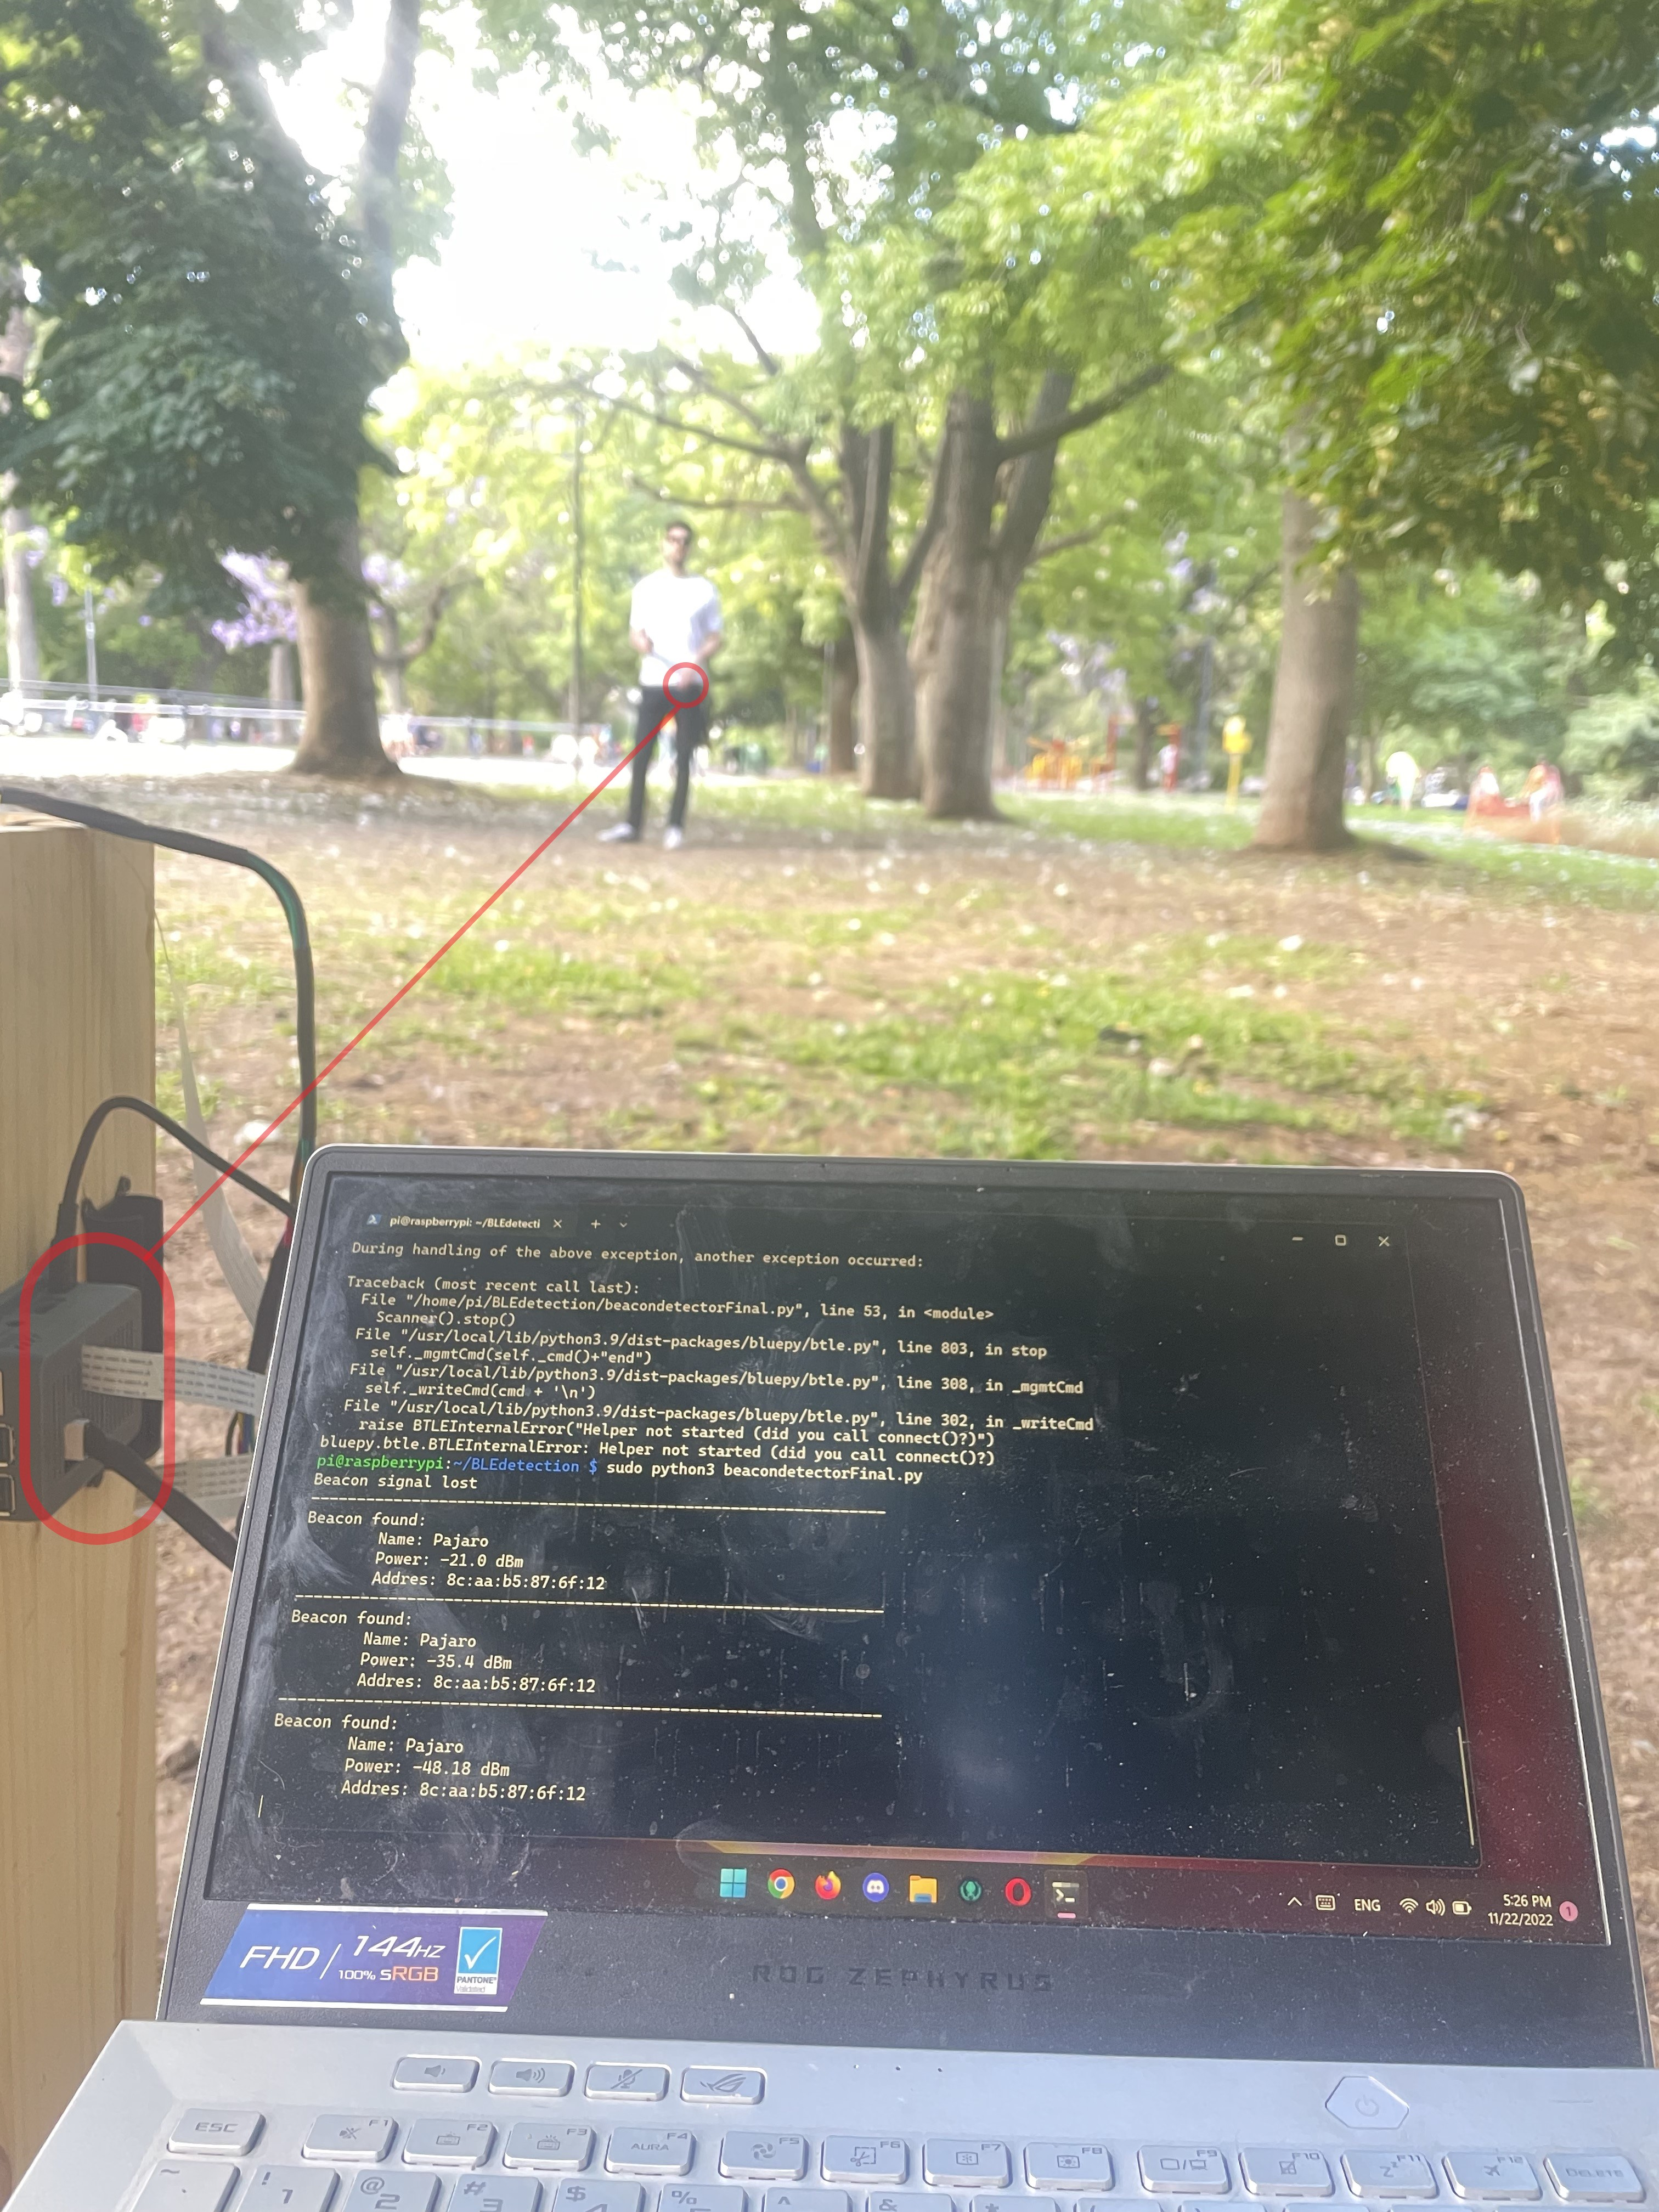
\includegraphics[width=\linewidth]{ImagenesValidacion del prototipo/TINTCOM12ba}		
		\caption{Distancia de 15 metros.}
	\end{subfigure}\hspace*{2.5cm}
	\begin{subfigure}{0.3\textwidth}
		\centering
		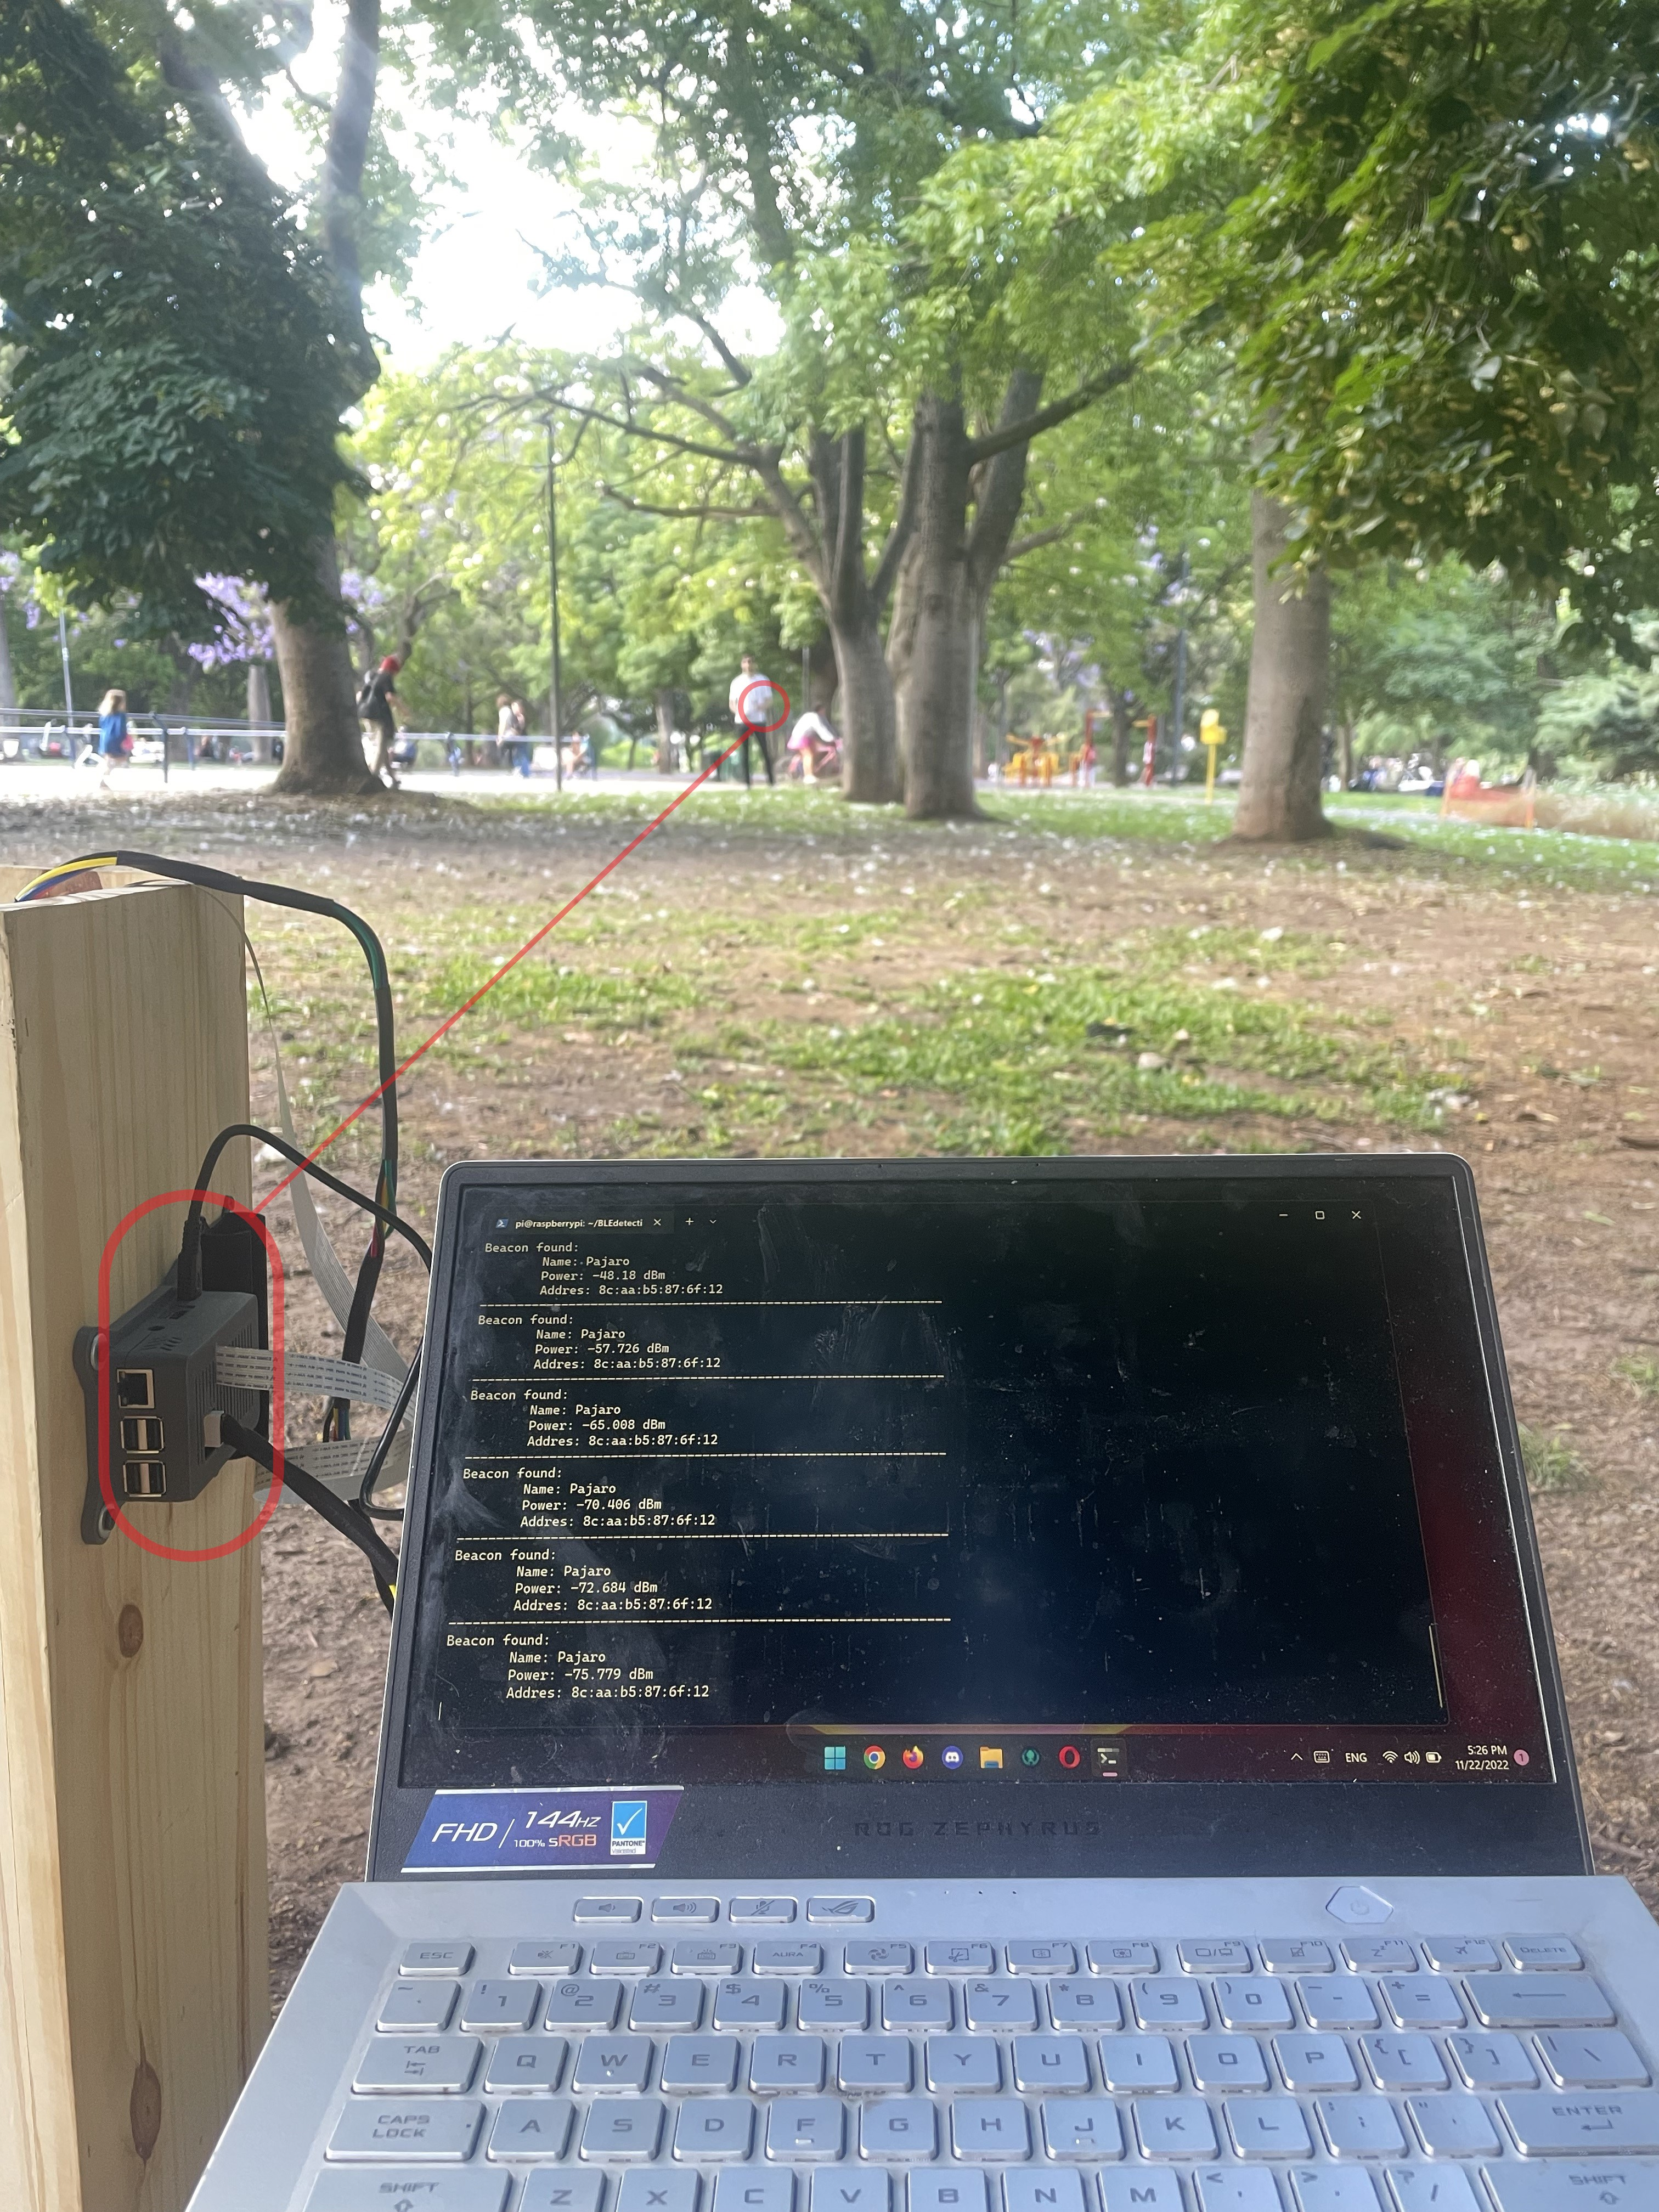
\includegraphics[width=\linewidth]{ImagenesValidacion del prototipo/TINTCOM12ca}
		\caption{Distancia de 30 metros.}
	\end{subfigure}
	\caption{Validación \textit{T-COM1-02}.}
\end{figure}

\Subsection{Validación Pruebas de Comunicación 2}
Para las pruebas de Comunicación 2 se requiere la computadora de un tercero (biólogo en campo). La primera prueba corresponde a \textit{T-INT-COM2-01} la cual consta en analizar a la capacidad de acceder a los datos del ave guardados en el nido.
\begin{figure}[H]
	\centering
	\begin{subfigure}{0.49\textwidth}
		\centering
		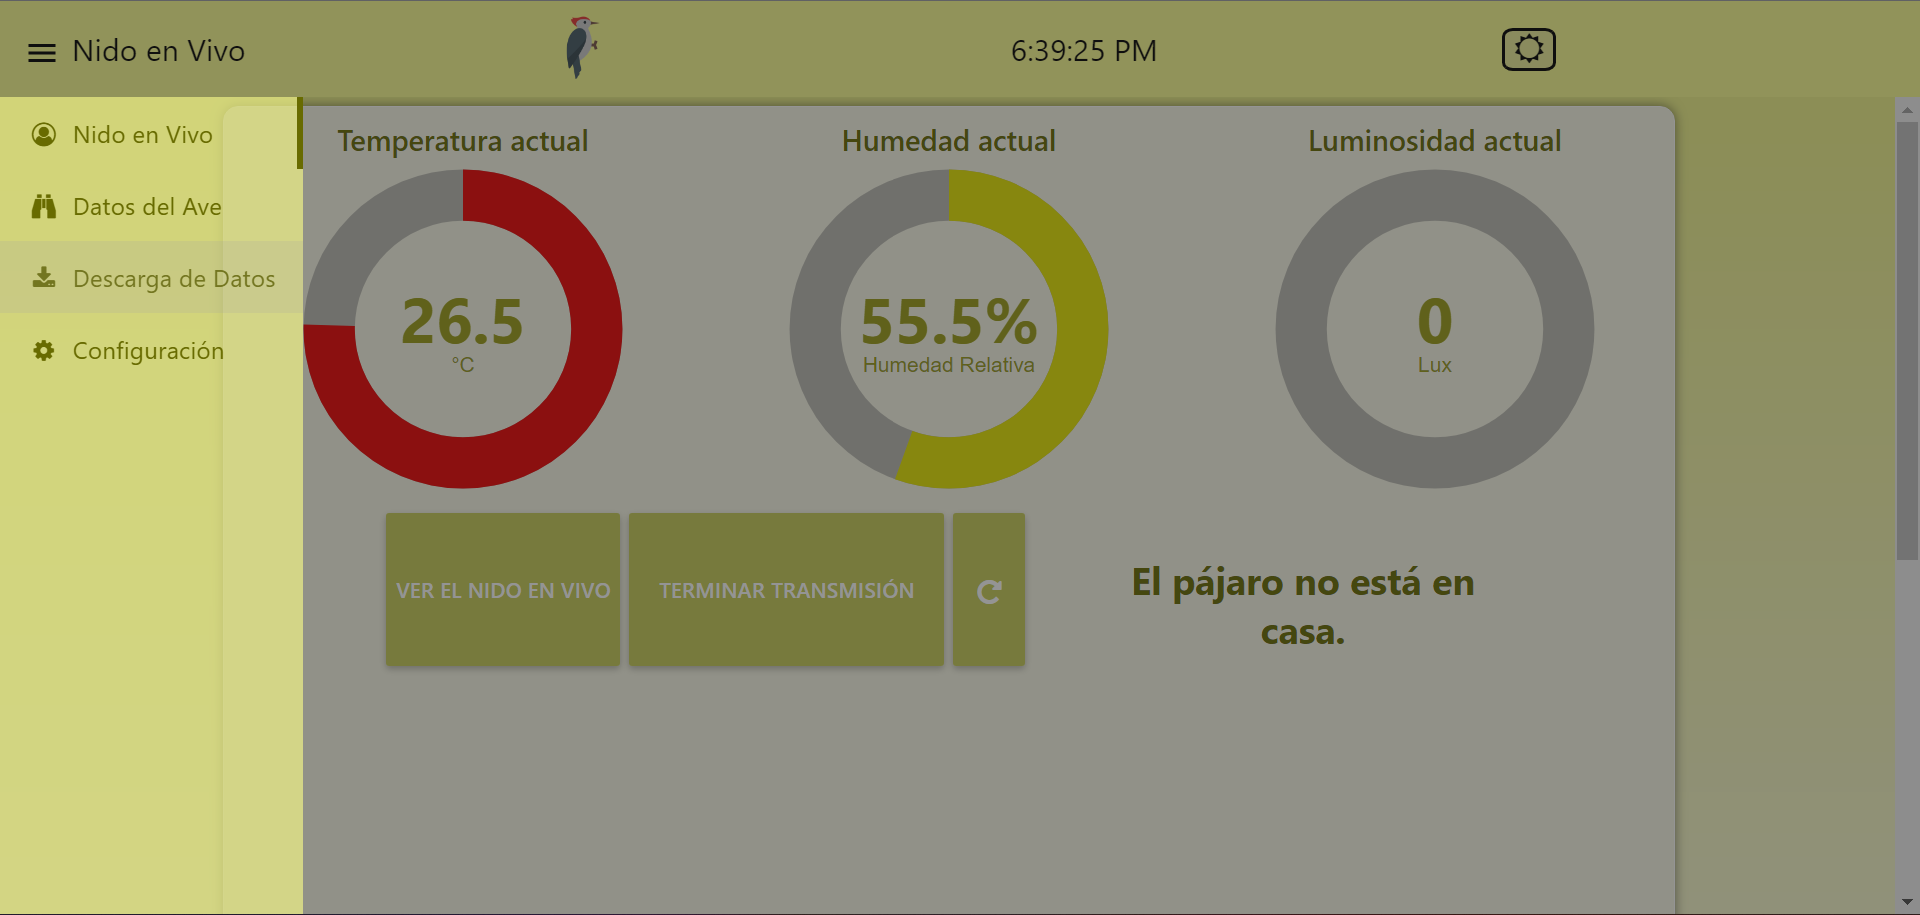
\includegraphics[width=\linewidth]{ImagenesValidacion del prototipo/TINTCOM21a}		
		\caption{Pestaña de descargas.}
	\end{subfigure}\hfill
	\begin{subfigure}{0.49\textwidth}
		\centering
		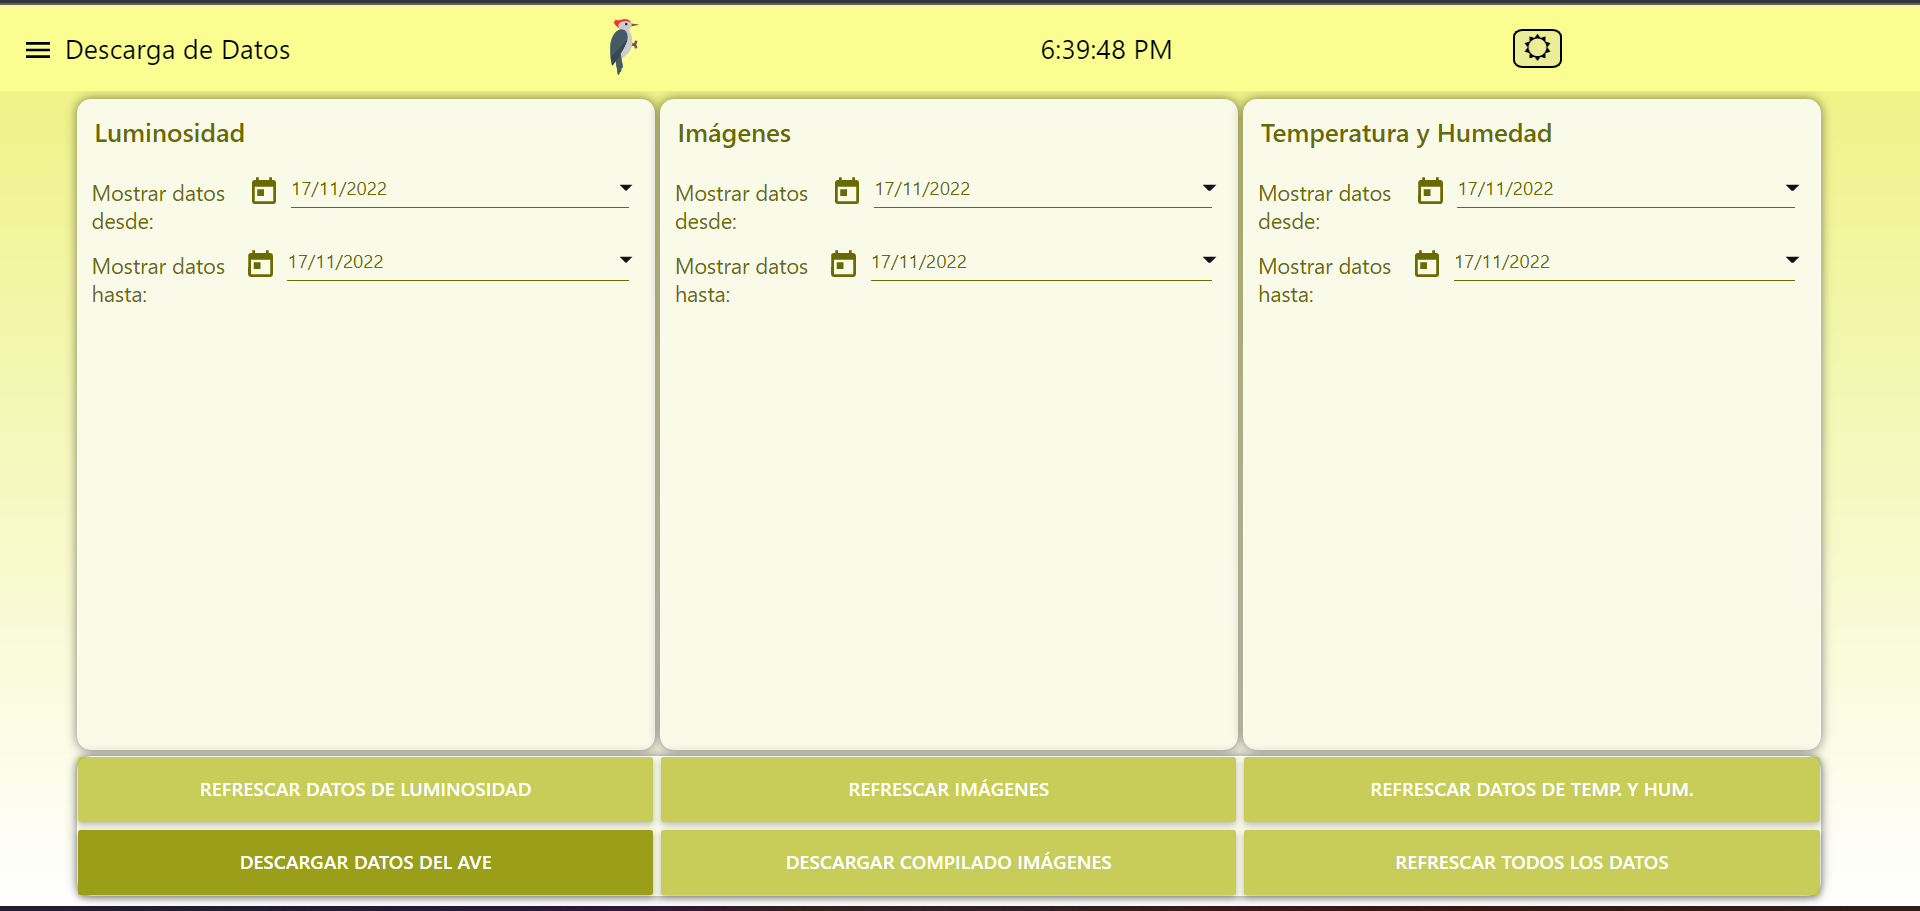
\includegraphics[width=\linewidth]{ImagenesValidacion del prototipo/TINTCOM21b}
		\caption{Botón de descarga.}
	\end{subfigure}
	\caption*{}
\end{figure}
\begin{figure}[H]
	\ContinuedFloat
	\centering
	\begin{subfigure}{\textwidth}
		\centering
		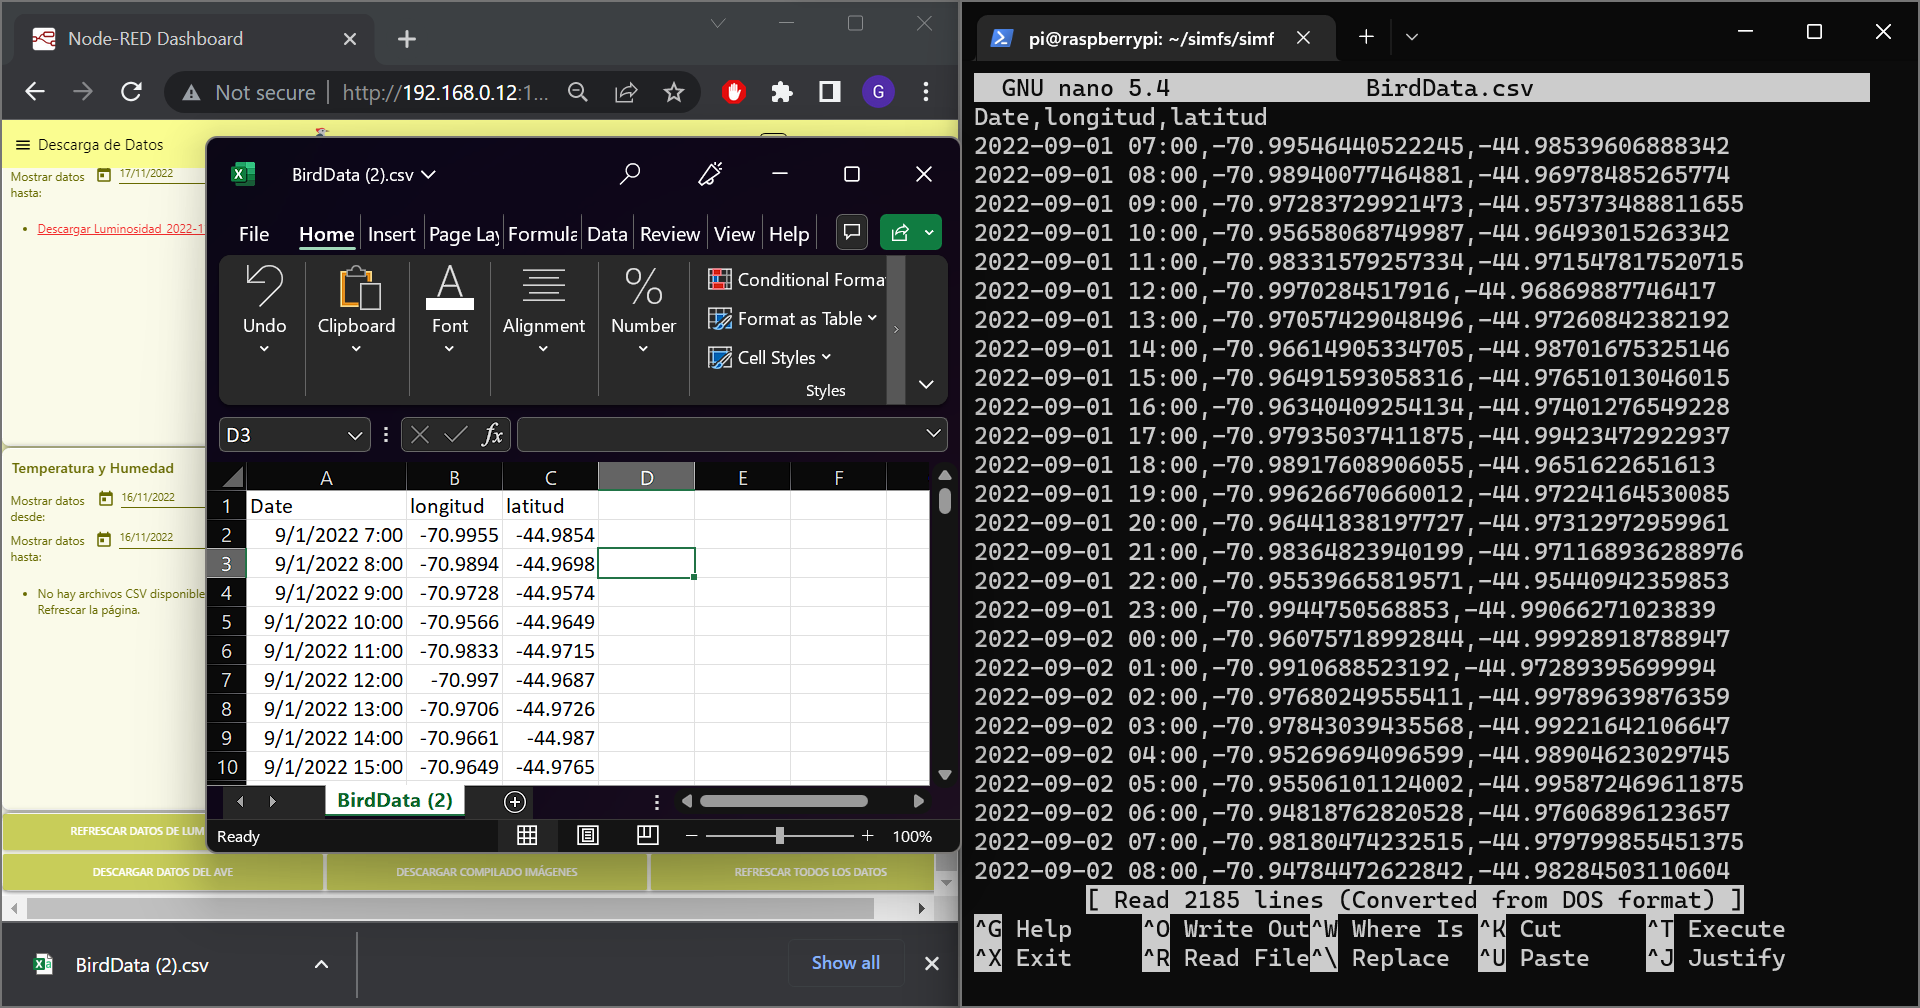
\includegraphics[width=0.8\linewidth]{ImagenesValidacion del prototipo/TINTCOM21}
		\caption{Consola y csv descargado.}
	\end{subfigure}
	\caption{Validación de comunicación \textit{T-INT-COM2-01}.}
\end{figure}

Se observa que los datos descargados que se ven en la izquierda se corresponden con los datos que se encuentran en el nido como se ve a la derecha. Por lo que no hubo una pérdida de datos.
Adicionalmente se utilizó una función de \textit{hash} para comparar los contenidos de ambos archivos y fehacientemente comprobar que son el mismo archivo. 

Por su parte, el desarrollo de las pruebas de \textit{T-INT-COM2-02} se efectuó sin mayores inconvenientes, logrando la conexión continua variando la distancia en rango de 4 a 14 metros.
\begin{figure}[H]
\centering	\includegraphics[width=0.55\linewidth]{ImagenesValidacion del prototipo/TINTCOM22}
	\caption{Validación de funcionalidad \textit{T-INT-COM2-02}.}
\end{figure}

Finalmente con lo que respecta a los bancos de prueba de comunicación, se procede a realizar la validación correspondiente a \textit{T-INT-COM2-03}. En esta prueba se de verificar la existencia del archivo \textit{BirdData} luego descargarlo y al acceder nuevamente a la \rspi comprobar que este fue borrado exitosamente.
\begin{figure}[H]
\centering
	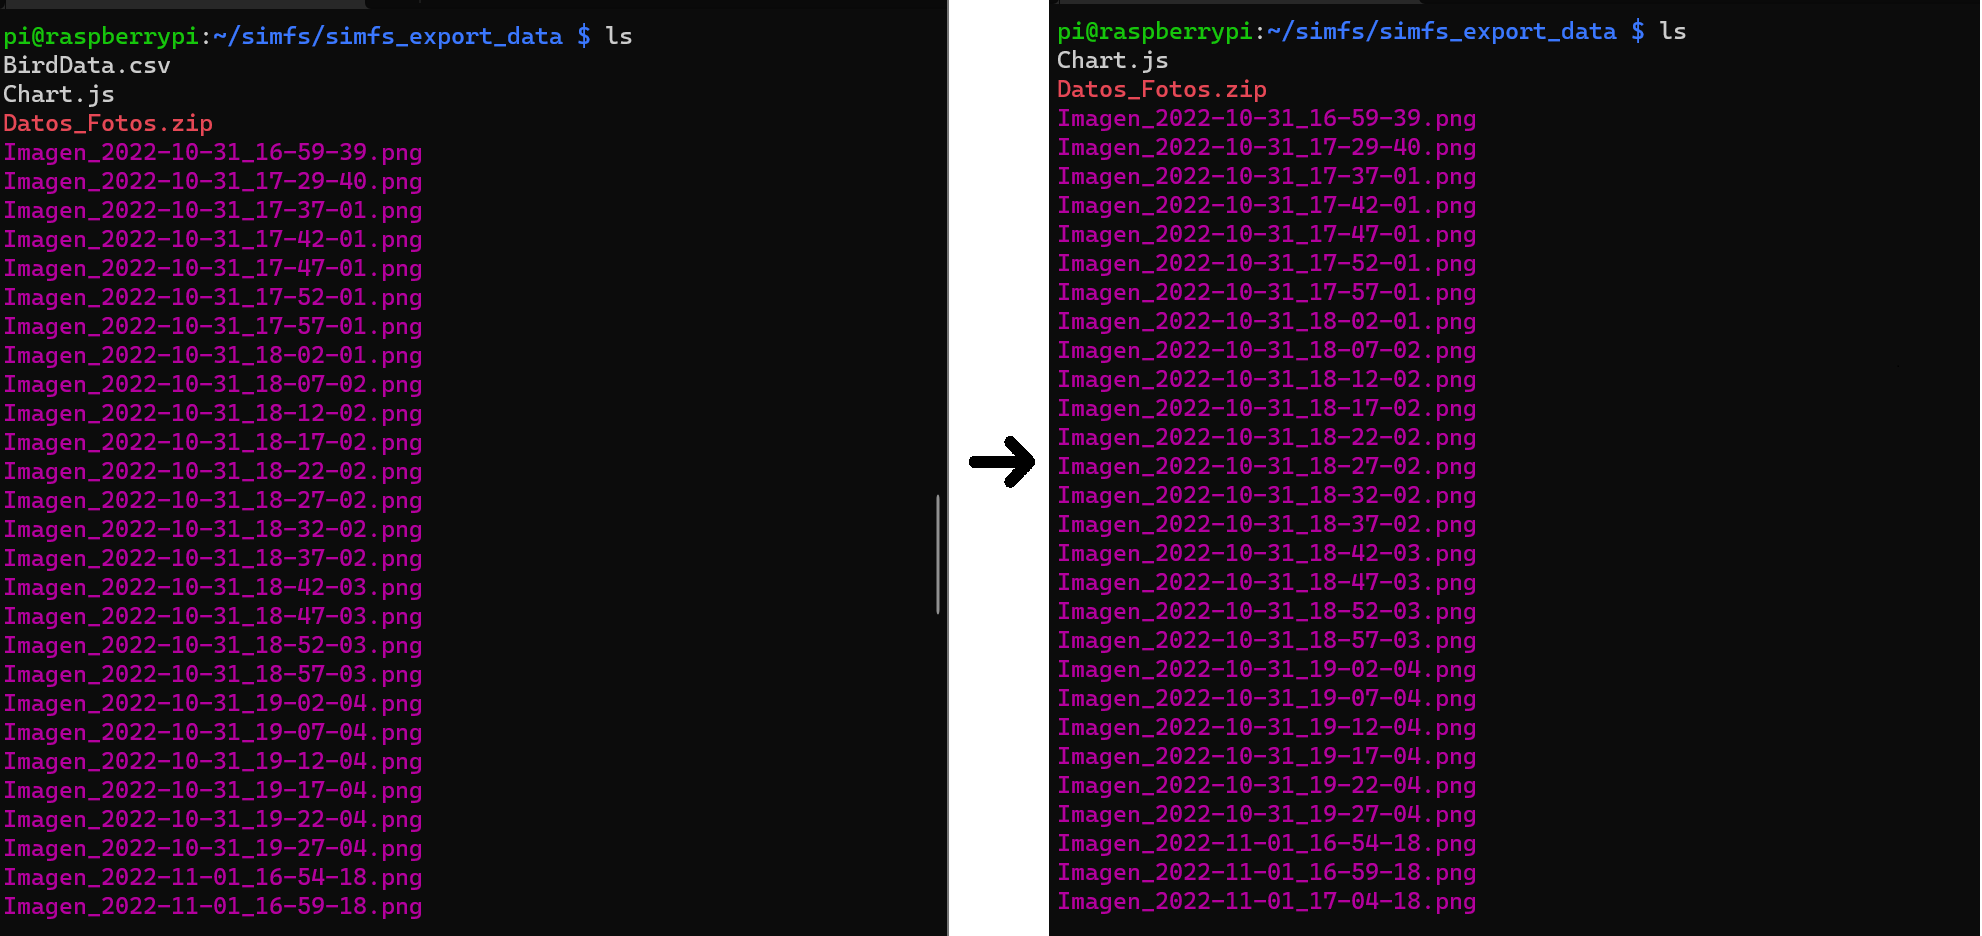
\includegraphics[width=1\linewidth]{ImagenesValidacion del prototipo/TINTCOM23}
	\caption{Validación de comunicación \textit{T-INT-COM2-3}.}
\end{figure}

\Subsection{Validación pruebas de seguridad}
Se dispuso del banco de pruebas \#1 para analizar la aplicabilidad de \textit{T-RAM-SEG-01}. El acceso tanto a la interfaz gráfica del usuario como la del administrador se encuentran restringidas para cualquiera que no posea las credenciales adecuadas.
\begin{figure}[H]
\centering
    	\begin{subfigure}{0.49\textwidth}
        	\centering
        	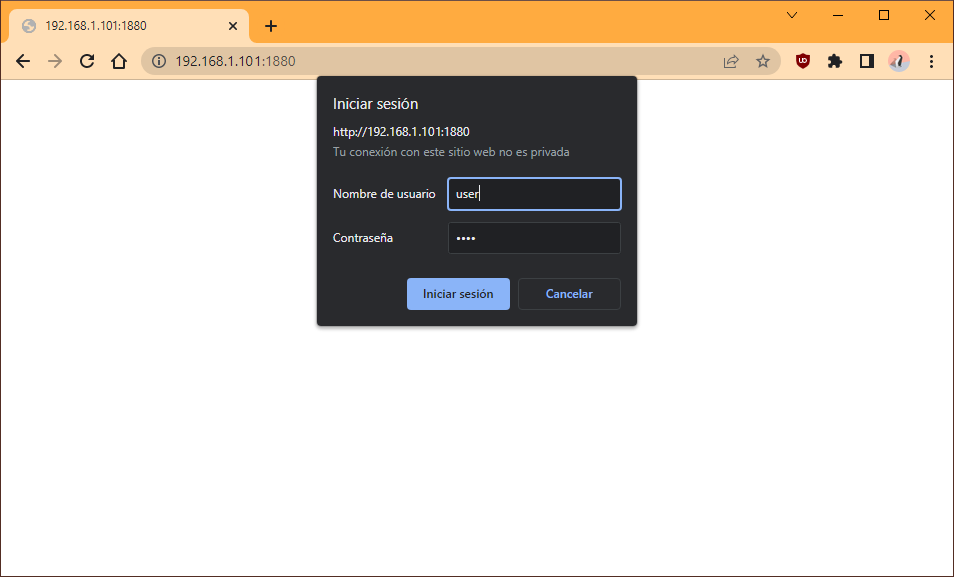
\includegraphics[width=\linewidth]{ImagenesValidacion del prototipo/t-ram-seg-01-1}		
			\caption{Autenticación de usuario para la interfaz gráfica.}
        \end{subfigure}\hfill
        \begin{subfigure}{0.49\textwidth}
        	\centering
        	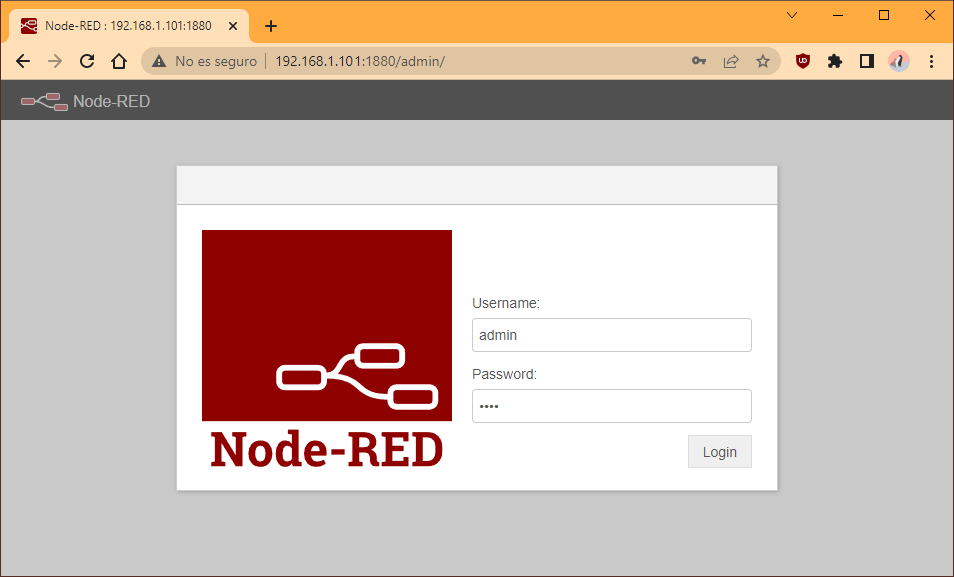
\includegraphics[width=\linewidth]{ImagenesValidacion del prototipo/t-ram-seg-01-2}
        	\caption{Autenticación de administrador para la interfaz gráfica.}
        \end{subfigure}
	\caption{Validación de seguridad \textit{T-RAM-SEG-01}.}
\end{figure}

Se obtuvo un resultado mejor del esperado ya que el hecho de emplear una red WiFi para conectar la unidad del nido con el usuario también requiere del uso de una contraseña. Esto agrega una capa de seguridad extra al sistema.
